%%% The main file. It contains definitions of basic parameters and includes all other parts.

%% Settings for single-side (simplex) printing
% Margins: left 40mm, right 25mm, top and bottom 25mm
% (but beware, LaTeX adds 1in implicitly)
\documentclass[12pt,a4paper]{report}
\setlength\textwidth{145mm}
\setlength\textheight{247mm}
\setlength\oddsidemargin{15mm}
\setlength\evensidemargin{15mm}
\setlength\topmargin{0mm}
\setlength\headsep{0mm}
\setlength\headheight{0mm}
% \openright makes the following text appear on a right-hand page
\let\openright=\clearpage

%% Settings for two-sided (duplex) printing
% \documentclass[12pt,a4paper,twoside,openright]{report}
% \setlength\textwidth{145mm}
% \setlength\textheight{247mm}
% \setlength\oddsidemargin{14.2mm}
% \setlength\evensidemargin{0mm}
% \setlength\topmargin{0mm}
% \setlength\headsep{0mm}
% \setlength\headheight{0mm}
% \let\openright=\cleardoublepage

%% Generate PDF/A-2u
\usepackage[a-2u]{pdfx}

%% Character encoding: usually latin2, cp1250 or utf8:
\usepackage[utf8]{inputenc}

%% Prefer Latin Modern fonts
\usepackage{lmodern}

%% Further useful packages (included in most LaTeX distributions)
\usepackage{amsmath}        % extensions for typesetting of math
\usepackage{amsfonts}       % math fonts
\usepackage{amsthm}         % theorems, definitions, etc.
\usepackage{bbding}         % various symbols (squares, asterisks, scissors, ...)
\usepackage{bm}             % boldface symbols (\bm)
\usepackage{graphicx}       % embedding of pictures
\usepackage{fancyvrb}       % improved verbatim environment
\usepackage{natbib}         % citation style AUTHOR (YEAR), or AUTHOR [NUMBER]
\usepackage[nottoc]{tocbibind} % makes sure that bibliography and the lists
			    % of figures/tables are included in the table
			    % of contents
\usepackage{dcolumn}        % improved alignment of table columns
\usepackage{booktabs}       % improved horizontal lines in tables
\usepackage{paralist}       % improved enumerate and itemize
\usepackage[usenames]{xcolor}  % typesetting in color

%%% Basic information on the thesis

% Thesis title in English (exactly as in the formal assignment)
\def\ThesisTitle{Extracting Information from Database Modeling Tools}

% Author of the thesis
\def\ThesisAuthor{Denis Drobný}

% Year when the thesis is submitted
\def\YearSubmitted{2019}

% Name of the department or institute, where the work was officially assigned
% (according to the Organizational Structure of MFF UK in English,
% or a full name of a department outside MFF)
\def\Department{Department of Distributed and Dependable Systems}

% Is it a department (katedra), or an institute (ústav)?
\def\DeptType{Department}

% Thesis supervisor: name, surname and titles
\def\Supervisor{RNDr. Pavel Parízek, Ph.D.}

% Supervisor's department (again according to Organizational structure of MFF)
\def\SupervisorsDepartment{Department of Distributed and Dependable Systems}

% Study programme and specialization
\def\StudyProgramme{Computer Science}
\def\StudyBranch{Programming and Software Systems}

% An optional dedication: you can thank whomever you wish (your supervisor,
% consultant, a person who lent the software, etc.)
\def\Dedication{%
Dedication.
}

% Abstract (recommended length around 80-200 words; this is not a copy of your thesis assignment!)
\def\Abstract{%
Data lineage is a way of showing how information flows through complicated software systems. If the given system is a database, tables and columns are visualized along with SQL transformations of the stored data. However, this picture may be difficult to understand for people with weaker technical background, as database objects usually obey naming conventions and do not necessarily represent something tangible. To improve lineage comprehension, we developed a software called Metadata Extractor that on one hand brings further description of the database objects, as well as introduces a whole new perspective on data in a system through business lineage aimed for non-technical users. The additional metadata enriching data lineage are extracted from data modeling tools, such as ER/Studio and PowerDesigner, that are widely used in database design process. 
The solution extends the Manta Flow lineage tool, while taking advantage of its features at the same time. \\
}

% 3 to 5 keywords (recommended), each enclosed in curly braces
\def\Keywords{%
{Data Lineage}, {Data Modeling}, {Database Architecture}, {\TODO{Metadata}}
}

%% The hyperref package for clickable links in PDF and also for storing
%% metadata to PDF (including the table of contents).
%% Most settings are pre-set by the pdfx package.
\hypersetup{unicode}
\hypersetup{breaklinks=true}

% Definitions of macros (see description inside)
%%% This file contains definitions of various useful macros and environments %%%
%%% Please add more macros here instead of cluttering other files with them. %%%

%%% Minor tweaks of style

% Macro for things that need to be done
\usepackage{xcolor}
\usepackage{tabto}
\usepackage{float}
\usepackage{tikz}
\usepackage{cleveref}
\usepackage{hyperref}
\newcommand\TODO[1]{\textcolor{red}{#1}}
\newcommand\definition[1]{\emph{#1}}
\newcommand{\classname}[1]{\texttt{#1}}
\newcommand{\methodname}[1]{\texttt{#1}}

% These macros employ a little dirty trick to convince LaTeX to typeset
% chapter headings sanely, without lots of empty space above them.
% Feel free to ignore.
\makeatletter
\def\@makechapterhead#1{
  {\parindent \z@ \raggedright \normalfont
   \Huge\bfseries \thechapter. #1
   \par\nobreak
   \vskip 20\p@
}}
\def\@makeschapterhead#1{
  {\parindent \z@ \raggedright \normalfont
   \Huge\bfseries #1
   \par\nobreak
   \vskip 20\p@
}}
\makeatother

% This macro defines a chapter, which is not numbered, but is included
% in the table of contents.
\def\chapwithtoc#1{
\chapter*{#1}
\addcontentsline{toc}{chapter}{#1}
}

% Draw black "slugs" whenever a line overflows, so that we can spot it easily.
\overfullrule=1mm

%%% Macros for definitions, theorems, claims, examples, ... (requires amsthm package)

\theoremstyle{plain}
\newtheorem{thm}{Theorem}
\newtheorem{lemma}[thm]{Lemma}
\newtheorem{claim}[thm]{Claim}

\theoremstyle{plain}
\newtheorem{defn}{Definition}

\theoremstyle{remark}
\newtheorem*{cor}{Corollary}
\newtheorem*{rem}{Remark}
\newtheorem*{example}{Example}

%%% An environment for proofs

%%% FIXME %%% \newenvironment{proof}{
%%% FIXME %%%   \par\medskip\noindent
%%% FIXME %%%   \textit{Proof}.
%%% FIXME %%% }{
%%% FIXME %%% \newline
%%% FIXME %%% \rightline{$\square$}  % or \SquareCastShadowBottomRight from bbding package
%%% FIXME %%% }

%%% An environment for typesetting of program code and input/output
%%% of programs. (Requires the fancyvrb package -- fancy verbatim.)

\DefineVerbatimEnvironment{code}{Verbatim}{fontsize=\small, frame=single}

%%% The field of all real and natural numbers
\newcommand{\R}{\mathbb{R}}
\newcommand{\N}{\mathbb{N}}

%%% Useful operators for statistics and probability
\DeclareMathOperator{\pr}{\textsf{P}}
\DeclareMathOperator{\E}{\textsf{E}\,}
\DeclareMathOperator{\var}{\textrm{var}}
\DeclareMathOperator{\sd}{\textrm{sd}}

%%% Transposition of a vector/matrix
\newcommand{\T}[1]{#1^\top}

%%% Various math goodies
\newcommand{\goto}{\rightarrow}
\newcommand{\gotop}{\stackrel{P}{\longrightarrow}}
\newcommand{\maon}[1]{o(n^{#1})}
\newcommand{\abs}[1]{\left|{#1}\right|}
\newcommand{\dint}{\int_0^\tau\!\!\int_0^\tau}
\newcommand{\isqr}[1]{\frac{1}{\sqrt{#1}}}

%%% Various table goodies
\newcommand{\pulrad}[1]{\raisebox{1.5ex}[0pt]{#1}}
\newcommand{\mc}[1]{\multicolumn{1}{c}{#1}}


% Title page and various mandatory informational pages
\begin{document}
\sloppy
%%% Title page of the thesis and other mandatory pages

%%% Title page of the thesis

\pagestyle{empty}
\hypersetup{pageanchor=false}
\begin{center}

\centerline{\mbox{
\includegraphics[width=166mm]{../img/logo-en.pdf}}}

\vspace{-8mm}
\vfill

{\bf\Large BACHELOR THESIS}

\vfill

{\LARGE\ThesisAuthor}

\vspace{15mm}

{\LARGE\bfseries\ThesisTitle}

\vfill

\Department

\vfill

\begin{tabular}{rl}

Supervisor of the bachelor thesis: & \Supervisor \\
\noalign{\vspace{2mm}}
Study programme: & \StudyProgramme \\
\noalign{\vspace{2mm}}
Study branch: & \StudyBranch \\
\end{tabular}

\vfill

% Zde doplňte rok
Prague \YearSubmitted

\end{center}

\newpage

%%% Here should be a bound sheet included -- a signed copy of the "bachelor
%%% thesis assignment". This assignment is NOT a part of the electronic
%%% version of the thesis. DO NOT SCAN.

%%% A page with a solemn declaration to the bachelor thesis

\openright
\hypersetup{pageanchor=true}
\pagestyle{plain}
\pagenumbering{roman}
\vglue 0pt plus 1fill


\noindent

\medskip\noindent
I hereby declare that I have authored this thesis independently, and that all sources used are declared in accordance with the “Metodický pokyn o etické přípravě vysokoškolských závěrečných prací”. \\

I acknowledge that my thesis (work) is subject to the rights and obligations arising from Act No. 121/2000 Coll., on Copyright and Rights Related to Copyright and on Amendments to Certain Laws (the Copyright Act), as amended, (hereinafter as the "Copyright Act"), in particular § 35, and § 60 of the Copyright Act governing the school work. \\

With respect to the computer programs that are part of my thesis (work) and with respect to all documentation related to the computer programs ("software"), I hereby grant the so-called MIT License. 
The MIT License represents a license to use the software free of charge. I grant this license to every person interested in using the software. Each person is entitled to obtain a copy of the software (including the related documentation) without any limitation, and may, without limitation, use, copy, modify, merge, publish, distribute, sublicense and / or sell copies of the software, and allow any person to whom the software is further provided to exercise the aforementioned rights. Ways of using the software or the extent of this use are not limited in any way. \\ 

The person interested in using the software is obliged to attach the text of the license terms as follows: \\

Copyright (c) \textless year\textgreater \  \textless copyright holders\textgreater \\
Permission is hereby granted, free of charge, to any person
obtaining a copy of this software and associated documentation
files (the "Software"), to deal in the Software without
restriction, including without limitation the rights to use,
copy, modify, merge, publish, distribute, sub-license, and/or sell
copies of the Software, and to permit persons to whom the
Software is furnished to do so, subject to the following
conditions: \\
The above copyright notice and this permission notice shall be
included in all copies or substantial portions of the Software. \\
THE SOFTWARE IS PROVIDED "AS IS", WITHOUT WARRANTY OF ANY KIND,
EXPRESS OR IMPLIED, INCLUDING BUT NOT LIMITED TO THE WARRANTIES
OF MERCHANTABILITY, FITNESS FOR A PARTICULAR PURPOSE AND
NON-INFRINGEMENT. IN NO EVENT SHALL THE AUTHORS OR COPYRIGHT
HOLDERS BE LIABLE FOR ANY CLAIM, DAMAGES OR OTHER LIABILITY,
WHETHER IN AN ACTION OF CONTRACT, TORT OR OTHERWISE, ARISING
FROM, OUT OF OR IN CONNECTION WITH THE SOFTWARE OR THE USE OR
OTHER DEALINGS IN THE SOFTWARE. \\

\vspace{10mm}

\hbox{\hbox to 0.5\hsize{%
In Prague date ............	% FIXME!
\hss}\hbox to 0.5\hsize{%
signature of the author
\hss}}

\vspace{20mm}
\newpage

%%% Dedication

\openright

\noindent
\Dedication

\newpage

%%% Mandatory information page of the thesis

\openright

\vbox to 0.5\vsize{
\setlength\parindent{0mm}
\setlength\parskip{5mm}

Title:
\ThesisTitle

Author:
\ThesisAuthor

\DeptType:
\Department

Supervisor:
\Supervisor, \SupervisorsDepartment

Abstract:
\Abstract

Keywords:
\Keywords

\vss}\newpage\vbox to 0.5\vsize{
\setlength\parindent{0mm}
\setlength\parskip{5mm}

Název práce:
\NazevPrace

Autor:
\ThesisAuthor

\TypPracoviste:
\Katedra

Vedoucí bakalářské práce:
\Vedouci, \KatedraVedouciho

Abstrakt:
\Abstrakt

Klíčová slova:
\KlicovaSlova

\vss}

\newpage

\openright
\pagestyle{plain}
\pagenumbering{arabic}
\setcounter{page}{1}


%%% A page with automatically generated table of contents of the bachelor thesis

\tableofcontents

%%% Each chapter is kept in a separate file
\chapter{Introduction}

There is no business today that can live without being backed by a database.
No matter what field an enterprise is focused on, we can enumerate many reasons why a database storage helps a company to be more effective and its deployment is a good idea.
We will justify it using some examples of how databases are used through various business domains.

\begin{itemize}
	
	\item Social Media \\
	Every piece of information that has ever been published on social media, from photo through a reaction or comment to friendship establishment, was stored somewhere and that place is a database. Usually the database that a social platform uses does its job in a background. Nevertheless there may occur events when the data storage reminds of its presence as it did on the most recent outage of Facebook. \cite{Facebook19}.
	
	\item Healthcare \\
	Easy accessibility of large amount of patient's data is a main reason to deploy a database at doctor's office or a healthcare organization \cite{Healthcare13}. High discretion is a requirement when managing data of such sensitiveness.
	
	\item Finances \\
	\TODO{complete}
	
	\item E-commerce \\
	Every company that sells products online should use a database. The bare minimum is to store offered products themselves and keeping track of purchases that were done by users.
	
	
\end{itemize}
And the list goes on.
\\

Once the decision is made and the usefulness of a database for our business is proved, there may be still a long way until everything runs as expected and we can make use of all the advantages that data storage brings.

The database design phase comes in place then. By the nature of the problem, a top-down approach to the process is usually followed since at the start there is an enterprise knows what real life aspects need to be captured in a database. To convert this idea into a working solution, the company would hire a database designer. \\ \\
A discussion between an expert in the business domain where the enterprise operates and a database professional follows, in order to identify and collect requirements for the future system.
In that moment data modeling comes into play. 
Instead of a transcript of the conversation, better solution is to translate the debate into more intuitive and standardized piece of documentation, into a conceptual data model.
Once the initial model is created the next steps are going more and more toward an final implementation of the database. After, a database designer works on development of a logical model and the most high level concepts are transformed into the one that is combining high level perspective with more technical aspects, but the description of them remain independent of a database type. \\ \\
Finally, the organization of the database is pointed out and captured in a physical model of the analyzed system, from this point we have a solid documentation and it is straightforward to finally deploy a database that is described in the low-level model as is has one-to-one mapping with implementation itself. \\ \\

The process of development and deployment of a database consists of multiple stages as we have seen. At the beginning there is a high level view of why the database is needed and what purpose will it serve. Hopefully, in some time the result is that the data described in the initial step are stored physically at some server. 
This way the data can be accessed and processed.

But that is just the beginning. The importance of a database for an enterprise is not in how it is designed. What does really matter is that big companies have plenty of business processes managing contents of storage via scripts in an automated way. 

For example travel companies offering airplane tickets commonly increase price when there is not many spaces left for a trip. 
Thus when a customer buys a ticket, there is a logic that computes how the price of the remaining tickets should be raised and update the records in database representing the not taken tickets accordingly, so the valid information is shown to customers.
The logic takes places thanks to by SQL queries applied on a database.
As the amount of business processes grows, the ability to justify correctness of data decreases. 
Also once an error in data is found in such a big ecosystem, it may be very unpleasant to trace it as data are affected by possibly huge number of sources and transformations hidden in scripts.

Data lineage is the answer for the struggles with being overwhelmed by complexity of a big data solution. It brings an ease to seeing what and how is affecting data stored in databases.

The lineage of data shows database tables and transformations used for either writing or reading data from tables. It is really helpful, however not for everyone. 
We outlined that there are multiple perspectives on a database through data models, and every perspective has a different audience eg. the conceptual is for business people while the physical one is read by database engineers.
But when it comes to data lineage, it only displays the level of abstraction that is understood by database professionals, while people with not that good technical background that would want to make decisions based on how data flows in their system are not having an easy time trying to figure out what is going on in such data lineage.
That is why we want to bring the business data lineage, which is speaking the language of more enterprise people coping with data and making decisions related to them on daily basis. We assume  big companies approach database development responsibly, thus there exist a documentation of their systems in form of data models, we will try to reuse to bring the desired functionality.
\TODO{GDPR use-case}

\section{Goals}

\begin{itemize}
	\item Develop a component that extracts metadata from database models that were created using SAP PowerDesigner 
	\item Develop a component that extracts metadata from database models that were created using ER/Studio
	\item Provide a description by means of a programming language for a general scenario of metadata extraction from a data modeling tool output and passing the information to a data lineage tool
	\item Propagate data lineage acquired by analysis of how is database used and constructed to more abstract data models than is the physical one, to the logical and the conceptual models.
\end{itemize}

\TODO{Introduction to each of the following chapters once the final organization is known}

\section{Glossary}
A \definition{database} is a collection of related data. By data, we mean known facts that can be computerized and that have implicit meaning as stated in \TODO{literature instead Fundamentals of Database Systems} \cite{ElmasryNavathe15}. We will consider that a database stores data relevant to an enterprise at a host that can be accessed via network. \\

A \definition{data model} is a description of data, data relationships, data semantics, and consistency constraints. \label{DataModel} \\
 
A \definition{database schema} defines how is the database described in a data model actually constructed, specifying types of fields from data model. Represents an instance of a data model. \\

A \definition{diagram} is a graphical visualization of a data model. \\

A \definition{data modeling tool} is a software that allows a database designer to create data models. End user may use the tools for interactive previewing of the models' diagrams. \\

\definition{Data lineage} provides a picture of how data moves in some system across its components. It is a description of how data go from an origin through their transformations until they reach a destination. 
The ability of seeing graphically how data are used, what for, and what are the consequences of the usage in a system is a powerful tool for error tracing. \\


\chapter{On Database Background}

\section{Databases}

A standalone database is not very useful as it is only some physical storage that never changes. To take the full advantage of it we need some means to define, create, maintain and control access to the database. That is purpose of a software called \definition{Database Management System (DBMS)}.

We already described why we want to use a database and roughly mentioned what are the pieces of data that we want to save there. 
Now let's take a look at what are differences between in database implementations and what to take in account when comparing database technologies.
That may be helpful when choosing the best suitable option for some specific data set to store or to see how storing of great amount of structured information can be approached. \\ 

The basic division of databases types is simple and binary - they are either Relational or Non-Relational.

There are Database Management Systems build around both, Relational Database Management System (RDBMS)

\subsubsection{Relational Databases}
A \definition{Relational Database} is a set of tables. A table consists of rows (also records) and columns. We can see such table as an object whose attributes are represented by columns and instances by rows. 
The important aspect is that relational tables tables carry both data that need to be stored by user and the relationships between the data as well. 
To store an atomic piece of data about instance a proper column is filled with a value.
Whereas to capture a relationship between objects the concept of keys is used. \\
A \definition{Key} is a subset of table's columns used for identifying a record. \\
A \definition{Primary Key} is a Key that non-ambiguously identifies a record in table and is used when referring to the record. \\
A \definition{Foreign Key} is a Key that uniquely identifies a record from a table (may be the same or a different one). \\
They are known also as SQL databases by the language - \definition{Structured Query Language (SQL)} which is used in RDBMS for managing data.

To be concrete, the most widely used relational database management systems are Oracle, MySQL, Microsoft SQL Server, PostgreSQL, IBM Db2 in this order. \footnote{The database technologies usage statistics are based on data from the most up to date version of website db-engines.com \cite{DatabaseEnginesStatistics19}.}

In this work will focus only on the databases that are of the relational kind, even though there are also NoSQL or Non-relational databases that do not follow the relational paradigm. 

The main reason behind this is the fact that NoSQL databases have a flexible schema or are schema-less (there is no point in determining a database schema when data types of attributes or keys) modeling of these databases quite a new discipline and is hard to find an intersection among different approaches to NoSQL modeling.
Also concepts of higher abstraction models are omitted. \cite{NoSQLDatabaseModeling}

The fact to consider is that once a database is Relational we more or less know what to expect from it. The structure of these databases has a fixed skeleton. So a tool that would extract metadata from relational data models is potentially more powerful as it can be applied to more database technologies than a similar tool aimed for some specific type of Non-Relational database. 

Lastly, despite the Non-Relational may be growing in numbers and became a serious alternative, as it suits some use-cases better, the Relational still are, and in the near future will be, far more widely used.

\subsubsection{Means of Database Access}

Databases can be managed directly using Database Management Systems by a user who is using query language for accessing a database. 
However third party, or application, programs need also access the DBMS. 
In our work two types of programs will be connecting to databases when fetching metadata - modeling tools when undergoing a reverse-engineering process and Manta Flow in the extraction phase.
A solution is to provide them with an application programming interface (API) that provides a set of methods available in the programming language that the application program was written in, so it can use them.
Most commonly when the API is called its implementation translates the request so that to a specific DBMS driver that it is passed after understands it and performs the desired action. \\

A \definition{Connection String} is a textual information used to identify a data source and establish a connection with it. It it is made of pairs of keywords and values separated by semicolon, the keywords are parameters of the connection.

\paragraph{APIs to DBMS}
\begin{itemize}
	\item Open Database Connectivity (ODBC)\\
		General, language independent, ER/Studio, PowerDesigner
	\item Java Database Connectivity (JDBC)\\
		The Java ecosystem, Manta Flow, PowerDesigner
	\item ADO.NET\\
		.NET Framework
\end{itemize}

\section{Database Modeling}
\label{chap:database_modeling}

Modeling is a crucial phase of database design process.
Developing a database is just like building a house. 
Every one will agree that no construction work can go without solid design and documentation. 
It would sound a bit strange to hire construction workers straight ahead and tell them that we need a house that has 5 rooms, some toilets and expect a good result. Most probably some building would be produced, but we will agree that expectations and requirements of the later inhabitant could not be met properly.
Surely there are good reasons why the usual steps are followed strictly.
Let us move on from the analogy to the database domain. \\
When deploying a database from a scratch we may think of two short term advantages. Firstly, the time needed to have data stored somewhere would be much shorter and secondly the initial cost of the system could be lower. \\
But over time both of the advantages will most likely, if the database is not ridiculously small, get outnumbered by problems that will begin to appear. Maintenance of a poorly designed system (or not designed at all) is expansive and leads to numerous outages.\\

There are good reasons to why modeling has its place in a database development process:

\begin{itemize}
	\item Higher quality.\\ Modeling push to thorough definition of the modeled problem. Once we know what to solve and what is the scope, it is much easier to come with different solutions and justify which of the proposed approaches is the most suitable one.
	
	\item Costs reduction.\\ Errors are identified thus can be caught in early stages, when they are easy to fix.
	
	\item Better documentation.\\ Data models form a nice piece of it, they are understandable by each of the involved stakeholders. When someone tries to understand the system, he can choose a data model on an appropriate level of abstraction that will introduce him the important aspects of the problem that suits his knowledge and qualification.
	
	\item Correctness.\\ Tracking whether high-level concepts were implemented and represented correctly in the end is made straightforward.
	
	\item Determining of consistency of the system.
	
	\item Deeper understanding.\\ During the design process we may learn a lot about properties of the data that we need or have and will be stored. These information are crucial for choosing an appropriate type of database, whether to stick with a relational database if so which DBMS is the one for us, or to look for a non-relational one.
\end{itemize}

\subsection{Data Model Perspectives}

\subsubsection{Vertical Division}

American National Standards Institute \cite{ANSIArchitecture75} came with a database structure called Three-schema architecture. It is formed by:
\begin{itemize}
	\item External Level \\ Database as a user sees it, view of the conceptual level. 
	\item Conceptual Level \\ Point of view of the enterprise that the database belongs to.
	\item Physical Level \\ The actual implementation.
\end{itemize}

The idea behind the structure was to create three different views that are independent of each other. 
For example change of the implementation that is tied with physical level would not affect any of the remaining levels if the structures remained the same. 
The important aspect is that this structure is used to describe finished product, it does not say anything about the design process that leads to the product and should not be mistaken with the differentiation of data models that will be introduced.\\

On the other hand, to standardize process of designing a database Peter Chen\cite{Chen76theentity-relationship} identified four levels of view of data, where each of the levels has its important place: \\
\begin{enumerate}
	\item Information concerning entities and relationships which exist in our minds.
	\item Information structure-organization of information in which entities and relationships are represented by data.
	\item Access-path-independent\footnote{An \definition{access path} is a description how records stored in a database are retrieved by database management system\cite{AccessPathDefiniton}. The important part is that the path is specific for a DBMS technology.} data structure-the data structures which are not involved with search schemes, indexing schemes, etc.
	\item Access-path-dependent data structure.
\end{enumerate}

The categorization of data models have undergone some modifications, for example the first level is today omitted, to the one that is recognized nowadays. The differentiation takes takes into account  what is the audience that will work with a data model, whether it is someone who knows all about databases or a business person without technical background. The levels of abstraction used today\cite{SilberschatzKorthSudarshan10} are the following: 
\begin{itemize}
	\item Conceptual Data Models (High-Level) \\
	Reproduces real world objects along with their relationships and should be close to how business end-users perceive them.
	
	\item Logical Data Models (Implementation, Representational) \\
	In the middle between the two other model types there are representational data models which on the one hand are comprehensible by end-users and on the other hand are not too abstract so that they can be used as documentation for an actual database implementation of the modeled data.
	
	\item Physical Level Data Models(Low-Level) \\
	In contrast to conceptual models the physical ones are tied with how data are stored physically at storage media showing all specific internal details that may be overwhelming in the case that the reader is a computer specialist.
\end{itemize}


\subsubsection{Horizontal Division}

\subsubsection{Relational Data Model}

A relational database is a direct implementation of a relational data model. A reader should be already familiar with the concepts used in the models from the sections describing terminology of SQL databases. All the terms such as table, column, entity, record and keys originate in the definition of relational data model \cite{Codd69}.

\subsubsection{Entity-Relationship Data Model}

The \definition{entity-relationship (ER) data model} was the direct answer for the four level architecture\cite{Chen76theentity-relationship} that covers the highest two levels and may be a basis for unified view of data. \\
It was an opposition to the three major data models that were used - relational, network and entity set model. His aim was to bring a data model that would reflect real-world objects and relations between them naturally, while having advantages of all the three already existing models. The mission seems to be successful as years have proven the ER data model to be the most suitable one for conceptual data modeling. Moreover, ER data models are used most commonly in logical data modeling as well.

\subsubsection{Enhanced-Entity-Relationship Data Model}

An extended version of ER data model was introduced later - \definition{enhanced-entity-relationship (EER) data model}. The main change is that concept sub-classes and super-classes, known as inheritance or is-a relationship, between entities was brought. \\ 

\TODO{conclusion}
Conceptual and logical data models are usually represented by ER data models. 
The question is what specific data model type is used for physical models. 
As the most low-level model type is tied directly with how a database is organized, physical models must obey the structure of database.

\subsection{Conceptual Data Model}

The purpose of a conceptual data model is to project to the model real-world and business concepts or objects. \\

\subsubsection{Characteristics}
\begin{itemize}
	\item Aimed to be readable and understandable by everyone.
	\item Is completely independent of technicalities like a software used to manage the data, DBMS, data types etc.
	\item Is not normalized.
\end{itemize}

A real world object is captured by an \definition{entity} in conceptual model. \\
For further description of objects that we are interested in \definition{attributes} are used, those are properties of entities. Only the important ones are listed. \footnote{Definitions varies and in some literature can be even found that a conceptual entity lacks attributes. We assume that the entity can contain important attributes as it is more common interpretation and modeling tools have attributes support on conceptual layer as well.} \\
Also \definition{relationships} between objects are necessary to provide full view of the section of the world that a data model resembles. \\

To illustrate it on an example, if our modeling domain is education, then an entity may be a teacher or lesson. 
A lsalary number would be an information to store when describing teacher, making it an attribute.
Having lectures captured in our data model, it is really fundamental to see what lesson is taught by who, that would be captured using relationships.

\begin{figure}[H]
	\centering
	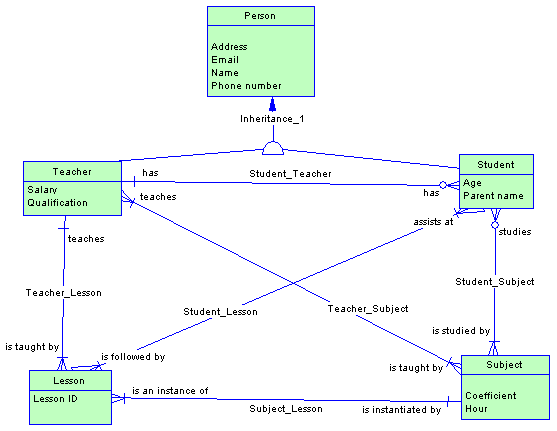
\includegraphics[width=10cm]{../img/Conceptual_Model_PowerDesigner}
	\caption{\TODO{Conceptual diagram}\cite{PowerDesignerDocumentation}}
\end{figure}

\subsection{Logical Data Model}

Keeping its structure generic a logical model extends the objects described in a conceptual data model making it not that easy to read but becomes a good base documentation for an implementation. Data requirements are described from business point of view.

\subsubsection{Characteristics}
\begin{itemize}
	\item Independent of a software used to manage the data or DBMS.
	\item Each entity has the primary key.
	\item Foreign keys are expressed.
	\item Data types description is introduced (but in a way that is not tied with any specific technology).
	\item Normalized up to \TODO{third normal form}.
\end{itemize}
\definition{Entities}, \definition{attributes} and \definition{relationships} from a conceptual model are present on this layer as well. Relationships are not that abstract as before and keys that actually make relationship happen between entities are added as their attributes.

\begin{figure}[H]
	\centering
	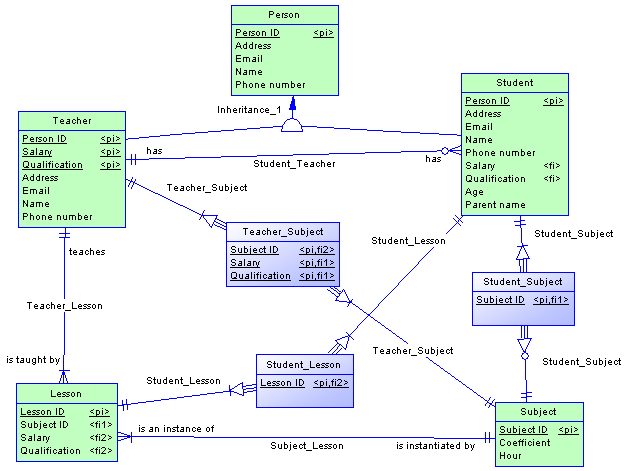
\includegraphics[width=10cm]{../img/Logical_Model_PowerDesigner}
	\caption{\TODO{Logical diagram}\cite{PowerDesignerDocumentation}}
\end{figure}

\subsection{Physical Data Model}

A physical data is a description of a database implementation so it is necessarily tied with one specific database technology as it should have one-to-one mapping to actual implementation. Its main message is to communicate how the data are stored.

\subsubsection{Characteristics}
\begin{itemize}
	\item Exact data types (DBMS specific) and default values of columns are outlined.
	\item DBMS's naming conventions are applied on objects.
	\item Constraints are defined (eg. not null, keys, or unique for columns).
	\item Contains validation rules, database triggers, indexes, stored procedures, domains, and access constraints.
	\item Normalization in order to avoid data redundancy or de-normalized if performance increase is reflected in the model.
\end{itemize}

Objects in physical models should reflect database organization and at the same moment related higher-level concepts should be transformable to physical level. \definition{Tables} should store records that corresponds to logical entities and \definition{columns} represent previously described attributes in memory.
Commonly schemas\footnote{Plural of the word schema is schemata but in literature about database design the word schemas is used} are present. A \definition{schema} is basically container for tables that logically groups them. Users have usually schemas assigned and can access only the tables contained in those schemas.

\begin{figure}[H]
	\centering
	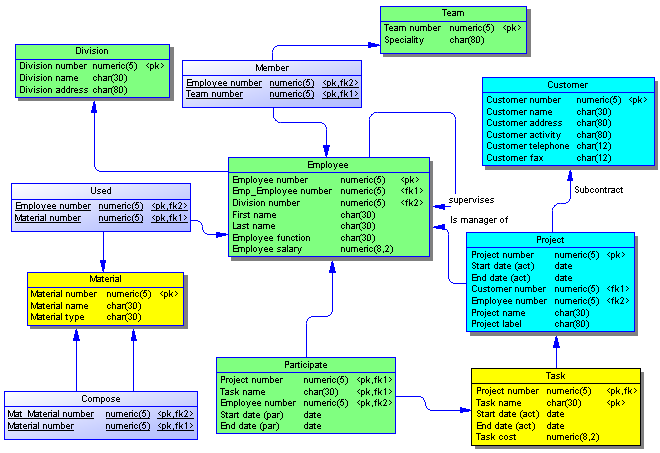
\includegraphics[width=10cm]{../img/Physical_Model_PowerDesigner}
	\caption{\TODO{Physical diagram}\cite{PowerDesignerDocumentation}}
\end{figure}

\subsection{Relations Between the Models}

We described what the role of each of the layers in a database design process is.
Now we will show that the data models are somehow connected vertically and what are the implications.

When talking about vertical divisions, we should think about how database design can proceed.

The basic approach is the \definition{top-down approach} to database modeling.
It is natural to start with a general idea what should a database store and what are the relations between stored object. 
End-user defines this high-level logic and as time goes importance of a database designer grows until he is at full charge and develops a complete database. It is the most common case of database development when a client identifies a high-level need for a database and hires an expert in this domain to make it happen.

The other way to create full view of a database is the \definition{bottom-up approach}. It can be harder to imagine what would be use-cases for this approach, but there are some problems that are bottom-up in nature. A nice real world example of bottom-up strategy is how doctors work. 
They start with "low-level" details such as symptoms and they're trying to build the whole image of patient's condition. So in the field of software data elements are firstly identified and after they are logically grouped to form bigger units, entities, and so on until the full hierarchy is known.

\subsubsection{Maps-to Relation}

In order to capture how high-level concepts are actually realized by more precise object a relation that we will call \definition{maps-to} is used. The relation leads between objects that are semantically equivalent on different levels of abstraction, sometimes even mapping between objects on the same layer are allowed but we will not consider this, as we consider it be mixing two different concepts together - data modeling with data lineage. To be more precise what we mean by semantically equivalent objects in data models is that we will assume maps-to edges solely source is model and target is model, entity and table, attribute and column, or the other way around.
Following these mapping links is extremely useful when a person wants to gain an overall overview of the system and comprehend it. For example when a user sees a data table in physical model that has a technical name that obey some naming convention and due to normalization does not represent any object straightforwardly, he can follow mapping links that leads to higher layer providing greater  abstraction over the implementation and the motivation why the table was created should be much clearer then.
It is worth mentioning that usually the mapping relations between objects of different layers simple one-to-one relationships but the cardinalities may vary greatly. For example one logical attribute may be realized via multiple database columns.
Normally more technical models are composed of bigger count of objects so one conceptual entity may be realized by multiple database tables in the end. Generally it is assumed that number of conceptual objects $<$ number of logical objects $<$ number of physical objects. It is natural that when capturing important high-level aims less entities is needed to express the intention but as we are getting closer to the implementation more necessary details come to play.
We consider the mapping relation symmetrical.

\section{Data Lineage}

\definition{Data lineage} brings a way of tracking data from its origin throughout the whole life cycle taking into account every process that manipulates the data until it reaches its final destination. It is like a telling the story of a piece of data including where does it come from and how it interacts with other data.
It should provide answers for questions where the data in given solution come from, whether it can be trusted or not, how it gets from point to point and how the data changes over time in the analyzed system.
Basically data lineage helps enterprises to gain deeper knowledge and understanding of what happens to data as it travels through various interconnected data pipelines\footnote{A pipeline is a set of elements manipulating and processing data where output of one element is input of another.} that the system consists of. Although we are focused on the subpart coping with databases, data lineage is a general concept where the sources and targets are not necessarily databases, data may come from, let's say, a user interface and ending in an output of a reporting software.
This overview of the system, that data lineage provides, is crucial when taking decisions about the infrastructure since the understanding of the consequences should more clear. Also it makes much easier to find errors in systems, since they can be tracked down from where the undesired behavior came to the surface to where the affected data originates. Surely somewhere between these two points the malfunctioning part is and thanks to data lineage the domain of suspicious operations should be reduced and visible. 
Therefore much time spent on solving issues should be saved.
Data lineage is a discipline of \definition{business intelligence}. \TODO{define}

To present data lineage a visual representation is most commonly used. Generally, we can think of the visualization as of a graph \TODO{explain graph elements}.

Having a reference point of interest we can divide data lineage into three types by what it captures. \definition{Forward data lineage} inspects movement of data towards the destination, \definition{backward data lineage} creates picture of what happened to data when traveling to the point from the source and the last type, \definition{end-to-end data lineage} combines both approaches and shows the full flow of data from its source until the very end destination.

Other differentiation of data lineage is the business one versus the technical one.
\definition{Business data lineage} highlights only transformations and aggregation of data in a simplified way to the target business user, whereas \definition{technical data lineage} displays precisely flow of physical data as is in underlying components (eg. applications) of the system is made of.

Now we will focus on how data lineage can be created to describe lifespan of data that are coming from or being saved to an SQL database.
To analyze flow of actual data, having access to quality metadata is fundamentally needed.
\definition{Metadata} are the data describing other data. The metadata we will use when analyzing a database are the likes of database name, names of tables, columns in tables, names of columns, procedures, data types etc.
When we have these information describing all the records that can be stored in the database together with all SQL scripts that are used for management of the database we can reliably determine how the data flows once the database is being used.

The idea of data lineage construction is as follows. First precondition is to have access to all metadata related to the database under analysis to have a clear picture of objects stored there. 
Then SQL queries that modify data are examined. They are stored in .sql files and usually a node is added for each of the files. We identify what tables and columns are the sources of input data for queries and where outputs of the operations are stored. Each input and output is represented by a graph node as well. Based on an analysis like this directed edges between the nodes we described are added to show dependencies. Inputs are connected with the query in such manner that every edges originates in of the input nodes and ends in the transformation node. Correspondingly, edges from query node to output nodes are made.

\TODO{an oversimplified example where data lineage would not be much of use as its importance grows with system's complexity.}



\subsection{Manta Flow}

Manta flow is a product of Czech startup company MANTA. It is a tool that automatizes data lineage creation by and analysis of programming code. It is able to cope with SQL, altogether with various of its sub-dialects, and Java. Uniqueness of the software is in its capability of handling code that is hardly readable by human. Thanks to this feature Manta Flow can automatically process databases consisting of millions of records and create a map of data flow across business intelligence environment - data lineage.
Alternatively the data flow is not visualized directly by Manta but cooperates with third party data governance solutions like Informatica, TopQuadrant, Collibra, IBM IGC etc. where it is integrated.

Our aim to interconnect the component that is subject of this work with Manta Flow to enrich the data lineage that it produces by metadata that can be obtained from relevant data models and can bring better understanding of the system under analysis.

\subsubsection{Supported Database Technologies}
Among other technologies currently Manta Flow is able to scan, these are the supported relational database types it can handle. 
That means when physical models are aimed on one of the following database types, we can create business lineage. Metadata Extractor is, naturally, effective on the same DBMS as Manta Flow. Specifically:
\begin{itemize}
	\item Oracle Database
	\item Microsoft SQL Server
	\item SAP ASE (Sybase)
	\item Hive
	\item IBM Netezza
	\item IBM DB2
	\item PostgreSQL
	\item Amazon Redshift
	\item Greenplum
\end{itemize}

\subsection{Data Lineage in Modeling Tools}

It is quite common that modeling tools provide some kind of view how data flow in the modeled diagrams or have data movement models where objects from data models take part. 
However this is not the way we will determine logical (or conceptual) data lineage.
The reason why not to take into account this feature is that it may be completely away from how really system works and data move. This is because none of the modeling tools inspects live databases and scripts working with them so the only way how a data lineage can be created in the tools is that a user draws this lineage by hand. 
It may be useful at the time when the database is not yet implemented and there is type of dependency relationship that cannot be captured other way. But once a database is running the lineage may get misleading as there is no way to enforce correctness of the data flows specified.
That is why we will bring a data lineage that corresponds to how a database is deployed and used in reality. Then thanks to mapping relations we can propagate the lineage to objects capturing more abstract concepts on conceptual and logical level where the lineage edges will be created by interpolation.
\chapter{Modeling Tools}
\label{modeling_tools}

The main feature of modeling tools is to capture metadata about data models that can be created using them and previewed. The tools use diagrams to present data models to their users.

\section{Construction of a Data Model}

Now we will take a look at how someone developing a database can actually create those models.
In fact, a data model could be created by hand using only paper and pen. It would definitely bring some of the benefits described above, but to take the full advantage of modeling, we assume using \definition{computer-aided software engineering (CASE) tools}. The tools are here to help with the development of quality software \cite{CASETools}. 
Here is an overview of different ways how a data model can be created using them.

\subsection{Modeling}

By modeling, we mean creating a data model via a user interface of CASE tools from scratch dragging a dropping data model objects around. 
This way of creation is the most similar to the pen and paper method. A user builds a model manually by selecting what object should be created and bringing it to the particular model, then he provides details about the object, creates sub-objects or specifies relationships with different objects.
Some tools do not allow creating an arbitrary model, but only the conceptual or logical models may be drawn like this. 
The reason behind not allowing user to create a physical data model out of scratch is that a physical model should either (i) be the result of a design process and be based on a model with higher level of abstraction (see \Cref{generating}) and then adjusted, or (ii) resemble a live database can be transformed into the corresponding data model by reverse-engineering (see \Cref{data_model_reverse_engineering}).

\subsection{Reverse Engineering}
\label{data_model_reverse_engineering}
Reverse engineering, or alternatively back engineering, is the process whose aim is to find out principles of how things are done or works in a system that is already running and try to gain a deeper understanding of the system.
Applied to our domain, the reverse engineering approach to the creation of a data model means that a CASE tool connects to a database and brings every object found to the physical model that is created. A database management system usually can provide additional metadata on objects, for example about primary/foreign keys, thanks to what relationships between tables, if the modeling tool is smart enough to make use of it, can be brought by the reverse-engineering process as well.
The model is an exact image of the database and one-to-one mapping between the model and database should be secured.

\subsection{Generating}
\label{generating}
Given a data model on some level, another model on different abstraction levels can be derived from it. Modeling tools usually support translating objects to semantically equivalent ones towards either greater or smaller abstraction. Of course, models created like this are not full-featured but they are definitely a better starting point for database designers to take over. 
For example, when a conceptual data model is arranged and a logical model should be created based on it, it is really helpful not to start from scratch. Instead, an outline of the logical model can be created by generating from a corresponding conceptual data model. 
Then it can be reshaped into the desired condition more quickly. 
Generation sources and targets are in maps-to relationship implicitly.

\subsection{Importing}
Finally, a CASE modeling tool may be able to import data models that were created using different modeling software and recreate the data models.

\section{ER/Studio Data Architect}

ER/Studio Data Architect is a data modeling and database architecture tool by IDERA, Inc. 
The latest version is 18.0 \cite{ErStudio}.

The tool is focused on building a business-driven data architecture providing an understandable interface for business users. It also improves data architecture standards by reducing redundancies, enforcing data consistency and quality.
The tool also tries to provide a framework for visualizing data flows by data lineage diagrams. 

ER/Studio supports creating logical and physical data models with the possibility of forward and reverse-engineering the models. Tens of database platforms can be targeted by a physical model.

The logical model is realized by an entity-relationship data model, whereas physical models are of a relational type.

The extension of the product, ER/Studio Data Architect Professional, comes with a model repository that makes collaborative development of data models easier. 

\section{PowerDesigner}

PowerDesigner is a software for data modeling owned by company SAP SE. The tool is well established and has been used by enterprises for 30 years, the current version is at 16.6~\cite{PowerDesignerHistory}.

PowerDesigner provides a range of various modeling techniques such as application UML modeling, business process description, enterprise architecture, data movements models and, most importantly, data modeling where conceptual, logical and physical data models are supported and physical models are compliant with more than 60 database management systems.
Forward and reverse-engineering of the models can be done.
The first two levels are of extended-entity-relationship data models and the physical one is of relational data model~\cite{PowerDesignerFeatures}.

The tool allows sharing metadata across all the supported model types and disposes of enterprise repository solution, which makes cooperative modeling by multiple users easy, has a version controlling ability and more.
\chapter{Analysis \& Design of the Solution}
\label{analysis_design}

The purpose of Metadata Extractor is to obtain metadata from data models that were created using modeling tools ER/Studio and PowerDesigner. 
The solution will be able to interact with Manta Flow and bring business lineage on objects from physical and logical data models. 
Currently, Manta Flow supports only the automated creation of technical lineage.

Here we describe how we proceeded when analyzing the solution and discuss crucial features of ER/Studio and PowerDesigner in detail.
Therefore, we can identify the important aspects of the tool that we needed to focus on when finally implementing Metadata Extractor.\\

In this chapter we provide answers to these questions:
\begin{enumerate}
	\item Identify what data models the modeling tools work with, what objects are contained in the supported data models, how they are organized and what metadata can be obtained that are relevant to be brought into data lineage.
	\item Find out how the data models are saved and how the interesting information from 1) can be reconstructed.
	\item Determine how the file format in what data models are stored can be parsed.
\end{enumerate}

\section{Analysis of the Problem}

We already presented that the modeling tools are capable of creating data models. These models are saved into files. 
The output files of the modeling tools are going to be the input of Metadata Extractor that uses them for the recreation of the objects and information contained in the data models.
In order to come with the logic of the reconstruction, we needed to identify what objects are saved in the files produced by modeling tools, and how they are represented. 
In \Cref{chap:database_modeling} about database modeling we introduced the standard layout of every data model type. We will quickly review their main objects. \\

\label{main_modeled_objects}
Conceptual and logical data models consist of entities, which may have attributes.
Physical data models are made of tables. A table is composed of columns that may belong to a schema.

These are the fundamental metadata Metadata Extractor must load form the files. 
Consequently, it must correctly load the hierarchy of these objects as it is modeled. For example, attributes must be assigned to entities correctly, etc.

Next, we look at how to find the pairs of objects that are in maps-to relation, and how do they refer to each other across levels of abstraction.
In an example, how a logical attribute and a physical column, are tied together across data models.

\subsection{File Format}

In this section, we firstly discuss what is the output of the analyzed modeling tools. Then we look at the main principles of how and what information is stored in the given format. Knowing this, Metadata Extractor can find the required objects (mentioned in \Cref{main_modeled_objects}) serialized in a file.

\subsubsection{ER/Studio}
\label{subsec:dm1_format}

The ER/Studio modeling tool uses its custom file format. These files have the .DM1 extension. 
In a single .DM1 file, related data models are stored. Let's call these models a solution. An \definition{ER/Studio solution} is a set of data models, describing a problem on both logical and physical levels (the two layers are only that ER/Studio supports). 
In such a solution one logical model must be present whereas 0 to N physical ones supporting the logical model.
We can imagine why ER/Studio behaves like this. The motivation may be that once there is a problem (if there is no challenge, no data modeling is needed), it must be described by a logical model. 
Possibly user has worked out the way to solve it, and that is when physical models are present as well.
Note that the actual storage may be distributed and the corresponding databases can be of different technologies, that is why more than one physical model are allowed in a single solution.

.DM1 is a textual file format that is organized into many tables.
Such a table is a CSV (comma-separated values) structure with modification since the file format consists of many of these tables, (i) each table has a unique name that identifies it. 
Next, (ii) a table contains a CSV row, which defines each column of the table. 
Lastly, (iii) CSV rows are standing for records that are stored in a table. 
To put it together, by a single table in .DM1 file we understand its name, column definitions, and records (rows representing data stored in the table).
At first sight, it is not clear how complex objects can be stored in files that we just described. To get the idea behind it, we did some work that we are going to describe in this section. 

\begin{figure}[H]
	\centering
	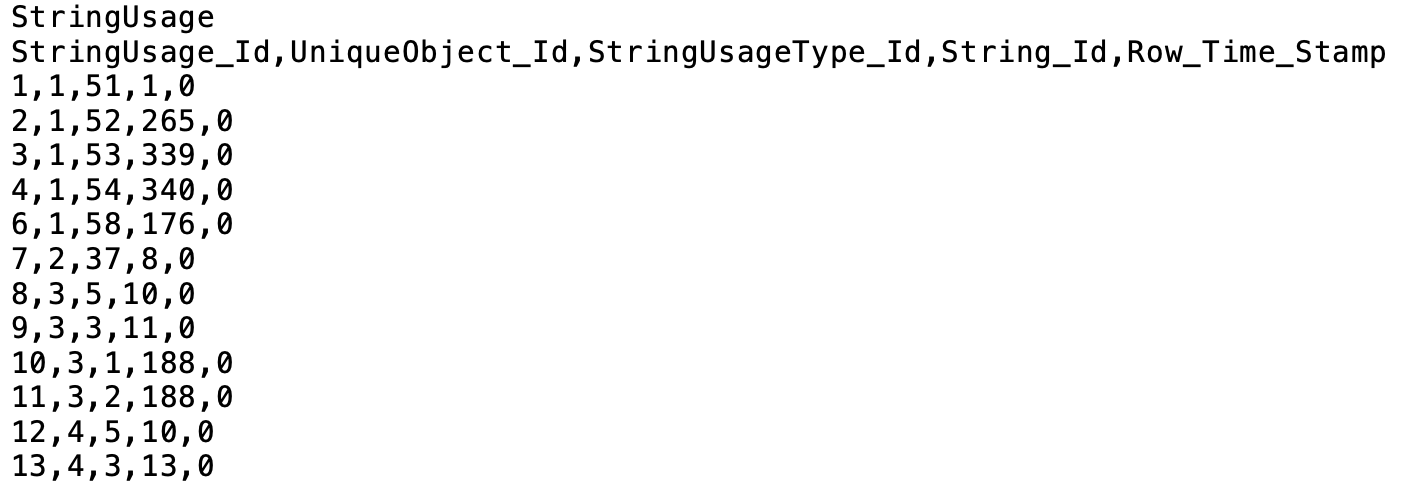
\includegraphics[width=14cm]{../img/StringUsageTable}
	\caption[Table from .DM1 file]{Example of a simple CSV table from a .DM1 file. It is named StringUsage, is made of five columns and stores 13 records.}
\end{figure}


An attentive reader may find the terms, we used for when describing a .DM1 table, familiar. 
As we already saw the terminology when introducing relational databases (see \Cref{relational_databases}). 
When going through the tables, we can notice columns that have common names.
That resembles primary and foreign key concepts used in relational databases, where a column is used to reference a record stored a different table. 
The keys indicate relations between tables.

It looks like this could be the answer to the question we proposed earlier - how complex objects can be stored in the simple tables. Each table stores a simple aspect of an object, but thanks to the relations, interconnected tables can be linked together and compose from their data a more complicated object.

To identify crucial relations that Metadata Extractor needs to know, in order to be able to reconstruct composite objects such as entities, attributes, etc., from .DM1 files, we developed a little reverse-engineering utility, which helps us to get an overview of the links between the tables.
Further details on how we proceeded when designing the utility can be found in \Cref{subsec:dm1_tool}. 

In order to work with a .DM1 file programmatically, it is needed to load it into suitable data structures that can be processed further. That is what a parser does. 
Metadata Extractor, as well as the reverse-engineering utility,  need such parser.
We mentioned the file format is basically a sequence of CSV tables. 
The question was whether to reach out for an existing CSV parsing solution or to develop a tailor-made one.
We took the second option, why and how we did so is described further in \Cref{subsec:dm1_parser}. \\

To sum up, the reverse-engineering utility provides an insight into the logic of .DM1 files, so Metadata Extractor knows what data model objects are stored in the files and how the complex objects are deserialized there. The parser prepares an input file, thus Metadata Extractor can reconstruct the objects and their metadata stored in it.

\subsubsection{PowerDesigner}

PowerDesigner produces files storing data models with three types of extensions - .pdm, .ldm and .cdm.
They stand for physical, logical and conceptual data models respectively.

While ER/Studio groups data models into solutions every model created in PowerDesigner is saved independently. 
A set of files that are at the same time opened in PowerDesigner forms its state. 
Such a state is called a workspace and can be saved into a .sws file. However, the workspace files do not bring us anything interesting. 
The information captured stores only what data models were at some time opened in the user's interface and does not tell anything about logical links between the files.

The data model files are XML (Extensible Markup Language) based file formats.
Alternatively, PowerDesigner is also able to save its data models into a binary file. The advantage is that the binary files can be processed more quickly and are smaller in size than the XML counterparts. 
However, we need a Metadata Extractor user to save his models as XMLs that is the only this way currently supported.

When parsing XML files there are two major ways how to do it. \\

The first approach is SAX (Simple API for XML), which is an event-driven parser that processes an XML document sequentially by a single pass. 
By default its processing is stateless and handlers are triggered when an event occurs. 
It is a simple and lightweight XML parser. \\

On the other hand, we have a family of DOM (Document Object Model) parsers. 
They load an XML file into a full AST (Abstract Syntactic Tree) structure. 
This way of file processing more memory and time consuming but translates everything stored in the input file into data structure straightforwardly. 
Then it can be conveniently worked with the tree-like resulting structure, where nodes represent parts of the processed document. \\

The great aspect of XML files is that they are human-readable and to figure out how the objects, Metadata Extractor is seeking, are serialized in these files is not that difficult.
In the next section, we describe what objects and information Metadata Extractor has to retrieve from the PowerDesigner data model files. We will see that the objects and their properties are quite complex.
Having a stateful parser would bring advantage as the context of the XML elements matter. For example, an element "name" that Metadata Extractor has to obtain can be attached to an entity, an attribute and many other kinds of objects.
Therefore, using a DOM parser is much more suitable and having the ability to do XPath queries over a DOM document is nicer than having to store a context manually, what would be needed to do with SAX.

\subsection{Metadata to Collect from Data Models}
\label{metadata_enumeration}

The main goal of Metadata Extractor is to bring business data lineage and to extract metadata for objects in both business data lineage and the technical one.
To meet the goal, we have to identify what objects and which of their metadata to collect from data models on every level of abstraction.

Metadata Extractor is aimed to bring information that is relevant to for data lineage and may be visualized when presenting a flow of data.
Modeling tools are exhaustive pieces of software with many features, thus have the ability to capture plenty of aspects that a modeled system has.
We determined types of information that can appear in data models of PowerDesigner and ER/Studio, makes sense to extract by analysis. Let us mention two important categories of metadata that we assume irrelevant to retrieve by Metadata Extractor.

Firstly, do not pay attention to relationships in the entity-relationship model. 
This is given by the nature of Manta Flow. It is not a modeling tool, thus it does not work with relations and edges between objects are used solely to represent a flow of data in a given system.
The only relationship type from data models we need to cope with is the inheritance relation, which is present in the enhanced-entity-relationship model. 
The difference is that without capturing the is-a links, an entity may not be described completely and the attributes that are inherited may be missing.

The second category of metadata that Metadata Extractor will ignore, are the ones that describe constraints on the actual data records saved in a database. 
Metadata Extractor works, just like Manta Flow, exclusively with database's metadata and does not access the data really saved in storage. 
Thus, our solution neither can monitor nor enforce any constraint on the database entries. 
That is why the metadata like keys or data types, which are also defined in data models, will not be in our domain of interest.

In this section, we list the specific types of objects we considered important for data lineage and what are the means to describe these objects even further by properties of theirs. 
The full list of metadata, including the ones we do not find useful to extract, is listed in \Cref{full_list_metadata}.

\subsubsection{Conceptual \& Logical Data Model}

Here we go through objects that appear in both conceptual and logical data models, together with what additional metadata can be attached to them.

\subsubsection{ER/Studio}

\subsubsection{CDM}

ER/Studio Data Architect does not support conceptual data models.

\subsubsection{LDM}

\begin{itemize}
	\item \entityname{Owner}: An owner is a concept equivalent to a schema - it is a container for logically related entities. Every entity belongs to an owner.
	\item \entityname{Entity}
	\begin{itemize}
		\item Name: The name of an entity.
		\item Attributes: Attributes assigned to an entity.
		\item Definition: Further description of an entity. Plain text or RTF (rich text format).
		\item Note: Notes are used when documentation about an entity is generated. Plain text or RTF.
		\item Where Used: This property shows objects that are in maps-to relation with an entity. Those which were created by generating.
		\item User-Defined Mappings: Shows objects that are in maps-to relation with an entity. These mappings are user-defined. They can contain a description of a relation, but we do not fetch the text as Manta Flow does not support attributes on mapping edges.
		\item Owner: The owner an entity belongs to.
	\end{itemize}
	\item \entityname{Attribute}
	\begin{itemize}
		\item Name
		\item Definition
		\item Notes
		\item Where Used
		\item User-Defined Mappings
	\end{itemize}
\end{itemize}


\subsubsection{PowerDesigner}

Conceptual and logical data models in PowerDesigner have so much in common that we propose a unified view on what may be stored in them. The properties/objects that are specific for either of them are marked with information in brackets saying "CDM/LDM only".

\subsubsection{CDM \& LDM}

\begin{itemize}
	\item \entityname{Data Item}(CDM only): A data item holds an elementary piece of information, which is given by some fact, or a definition, in a modeled system. It may or may not be present as a modeled object. Data items can be attached to entities to form their attributes. It is a datum that may seem relevant and is possible to capture at first but later may not be used as no entity needs it in the end.
	\begin{itemize}
		\item Name
		\item Code
		\item Comment: Plain text short description.
		\item Definition: An RTF description of an object.
		\item Annotation: A further RTF description.
		\item Keywords: Set of significant words specifying object's domain.
	\end{itemize}
	\item \entityname{Entity}
	\begin{itemize}
		\item Name 
		\item Attributes
		\item Code 
		\item Comment
		\item Definition
		\item Annotation
		\item Keywords
		\item Dependencies: Mapped entities.
	\end{itemize}
	\item \entityname{Attribute}
	\begin{itemize}
		\item Name 
		\item Code 
		\item Comment
		\item Definition
		\item Annotation
		\item Keywords
		\item Parent Entity
		\item Dependencies: Mapped attributes.
	\end{itemize}
	\item \entityname{Inheritance}
	\begin{itemize}
		\item Parent Entity: Predecessor.
		\item Child Entity: Inheriting entity that takes over attributes of the parent.
	\end{itemize}
\end{itemize}

\subsubsection{Physical Data Model}

In this section, we list objects from the physical level and their possible metadata.

\subsubsection{ER/Studio}

\begin{itemize}
	\item Type of Data Model: Database management system that a model is aimed for.
	\item \entityname{Schema}
	\begin{itemize}
		\item Name
		\item Tables
	\end{itemize}
	\item \entityname{Table}
	\begin{itemize}
		\item Name
		\item Columns
		\item Schema
		\item Definition
		\item Note
		\item Where Used
		\item User-Defined Mappings
	\end{itemize}
	\item \entityname{Column}
	\begin{itemize}
		\item Name
		\item Definition
		\item Notes
		\item Where Used
		\item User-Defined Mappings
	\end{itemize}
\end{itemize}

\subsubsection{PowerDesigner}

\begin{itemize}
	\item \entityname{Table}
	\begin{itemize}
		\item Name 
		\item Columns
		\item Code 
		\item Comment
		\item Definition
		\item Annotation
		\item Keywords
		\item Schema
		\item Dependencies
	\end{itemize}
	\item \entityname{Column}
	\begin{itemize}
		\item Name 
		\item Code 
		\item Comment
		\item Definition
		\item Annotation
		\item Keywords
		\item Table
		\item Dependencies
	\end{itemize}
\end{itemize}

\subsection{Reconstruction of Data Model}

Earlier in \Cref{metadata_enumeration} we defined what are the objects and their properties that Metadata Extractor must obtain from data models.
The objects living in the common environment of a data model, are related to each other into some kind of hierarchy.
The listing of the objects with their characteristics, which Metadata Extractor will retrieve from data models, makes us realize that the very basic layout of objects captured by a model resembles a tree-like structure.
The reason is that the analysis implies a general skeleton of a data model that goes like shown in \Cref{DataModelHierarchy}. However, it is just a simplified view. For example, data models do not need to support the concept of owners/schemas.

\begin{figure}[H]
	\centering
	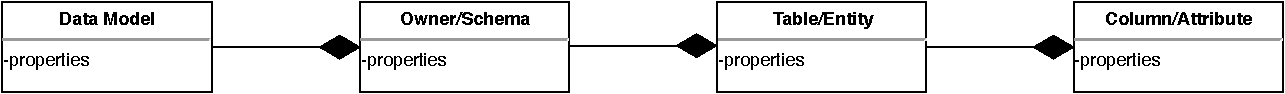
\includegraphics[width=14cm]{../img/DataModelHierarchy}
	\caption[Hierarchy of Objects in a Data Model]{General hierarchy of objects in a data model. The UML diagram pictures a data model that contains an arbitrary number of owners (schemas respectively), they own 0 to N tables (entities resp.), while each entity consists of zero or more columns (attributes resp.). These objects can be seen as nodes of a tree, whereas their properties are attributes of the corresponding nodes.}
	\label{DataModelHierarchy}
\end{figure} 

Surely further relations between the objects will come to play, like inheritances or mappings. They are going to be discussed later in the \Cref{maps_to_analysis}, making the diagram of objects in a data model more complex.

Metadata Extractor builds the tree from the top to the bottom. 
In the next two subsections, we describe how the main objects from \Cref{DataModelHierarchy} can be reconstructed from the output files of ER/Studio, PowerDesigner respectively.

\subsubsection{ER/Studio}

In the case of ER/Studio, each type of object is defined in a single table. Such a table stores all instances of the given type. 
An instance is identified in a table uniquely by its ID among other realizations of the same type.
Therefore, this ID is a primary key of a table. The relations from \Cref{DataModelHierarchy} are 
done by these keys.
An object has a reference to its, if we stick with the tree terminology, parent by storing parent's ID as a foreign key property of itself. 
Object's textual properties like name or definition are saved in a table containing string entries. 
Tables storing the records of the main objects, therefore, have also a column with foreign keys to the string table. 
So if Metadata Extractor proceeds by loading data models firstly, then descending down the tree, every time it is loading an object, its parent has already been constructed and the child can be simply plugged to the parent that the child references by a foreign key.

\subsubsection{PowerDesigner}

XML files form a tree structure by definition. This fact makes storing a hierarchy of objects with the same nature suitable and straightforward. 
This way a parent object of a child is simply its predecessor in the tree formed by XML elements of a file. 
Properties of an object are stored as child XML elements.
When Metadata Extractor creates the result, the top-down traversal of an XML tree is followed. 
At first, on its way down from the XML root, it builds objects higher in the hierarchy and only if a parent is built, Extractor examines its children. 
This way the context is clear and once, let's say an attribute, is created the program knows what is its parent entity trivially, as it must be the one that was created most recently.

\subsection{Maps-to Relation}
\label{maps_to_analysis}

Once we identified possible objects across the data models, it is really useful to know which objects are related, even though they were not defined at the same level of abstraction. 
It is important to keep the data models readable and to keep track of what tables are implementing which high-level concepts.

Our tool deals only with mappings of objects which are not at the same level of abstraction. 
Some modeling tools allow mapping, for example, a logical entity to a logical but it is unclear what is the meaning of such construct. 
One explanation would be that it expresses a relationship, but data modeling tools have other means available for defining relationships. 
Possibly, it could indicate that the entities are used identically as they are implemented by a single database table, but that is what data lineage describes precisely and will be brought by Metadata Extractor.

To be specific Metadata Extractor copes only with the following types mappings: 
\begin{itemize}
	\item An entity to a table or another entity. 
	\item An attribute to a column or another attribute.
\end{itemize}
\label{allowed_mappings}

Now we take a look at how the mappings are realized in the chosen data modeling tools.

\subsubsection{ER/Studio}

In \Cref{metadata_enumeration} we mentioned two types of mapping relations in ER/Studio for entities, tables, attributes, and columns.
In fact, the meaning of both types is the same. The only difference is that the where-used mappings are generated automatically, while the user-defined are drawn manually by a user. 
We assumed that all the objects that can appear in maps-to relation are in the very same solution, but there is also an option to create a mapping to objects which are defined in different .DM1 files. It can be done using the Compare and Merge utility in ER/Studio, whose functionality is to synchronize a model with another model/live database/SQL file. 
Among other operations that keep pairs in sync, there is the mapping creation option. 
We are interested in the first scenario, where the two compared data models may originate even in two different solutions. 
This, third, kind of maps-to relation is referred to as a universal mapping. \\

Knowing all the possible types of mapping relation, we will further focus on how they are saved in an ER/Studio .DM1 file and how can they be extracted. \\ 

Let's start with the seemingly easier case of mappings between objects inside the same ER/Studio solution - where-used and user-defined. 
After some analysis using the reverse-engineering tools (see \Cref{data_model_reverse_engineering}) we found the table that stores the mappings. It is named \erstudiotable{Where\textunderscore Used\textunderscore PD}.
In the table, there are four crucial attributes, IDs of the mapped objects and their Meta table types.
The first two attributes are foreign keys to tables, where the mapped objects are defined. The second pair of columns defines a type of the object so that Metadata Extractor knows to which tables it should look for the instances that are referenced by the foreign keys. 
The Meta table types also allow us to check, if the objects are actually compatible with each other in the sense of how we constrained the allowed mappings in \Cref{allowed_mappings}. \\

At first sight, solving the universal mappings may appear more difficult. It looks like Metadata Extractor will need to search for an object in different ER/Studio solutions and reconstruct the external objects. 
But the way the universal mappings are realized in ER/Studio is much simpler. 
Metadata Extractor does not need to open other files, as the external objects that are referenced by a universal mapping are stored in the analyzed .DM1 file. 
They are described briefly in a table called \erstudiotable{External\textunderscore Mapped\textunderscore Objects} by XML structures.
Metadata Extractor uses SAX parser to load these objects, as the XML object description is simple.
Finally, the table called \erstudiotable{Universal\textunderscore Mappings}, where all the mappings to external objects are defined is using the same concepts as \erstudiotable{Where\textunderscore Used\textunderscore PD} allowing Metadata Extractor to reconstruct them easily.

\subsubsection{PowerDesigner}

PowerDesigner saves every data model into a separate file. Therefore, to resolve mappings will be not as straightforward as in the case of ER/Studio, since every mapping of an object to another that is on a different abstraction layer leads across PowerDesigner files.
Firstly, let's go through the possible types of mappings, then we will discuss how to resolve the relation efficiently.

The mappings are divided into two categories. 
Similarly, as in the first tool, the mappings may be either generated or user-defined. \\ 


Before going through how the mappings are represented, we must mention the way objects taking part in the relation are identified.
Every important objects in PowerDesigner has a unique identifier named \elementname{ObjectID}. This sequence of characters is used when referring to the object.\\

When an object is created out of an existing one by generating, the resulting object has an XML element named \elementname{History}. The element contains holds all the IDs of objects that the final object was generated from.

User-defined mappings are represented by a composite XML element. 
The element representing a single mapping consists of a pair of mapped entities/tables IDs. If sub-objects of the pair are tied together by mapping as well, the XML element is a parent of further XML elements, which are specifying IDs of the underlying attributes/columns that are mapped to each other. \\

However, knowing the types of mappings and how they are saved in the PowerDesigner files is not enough to reconstruct the relation. Let's imagine the following scenario.
Metadata Extractor gets a file to process. It reconstructs objects stored in the file, then the program tries to resolve mappings, but one of the mapped objects is not accessible, as it is defined in a different file than is the one Metadata Extractor is currently reading.
Only the ID of the mapped counterpart is known. 
In order to gather all the required metadata about the mapped object, Metadata Extractor needs to find it by its ID in the file where it is defined.
Thus in a situation like this, the data model file is dependent on others.
In PowerDesigner's file format, Metadata Extractor can find an XML element describing targets of the given model, to learn what are the files it depends on.

When a model is generated from a file, such dependency is saved to both of the data model files, in the generation target as well as in the origin. 
In other words, if we imagine an oriented graph, where a file is a node and an edge leads from a file $a$ to file $b$ $\iff$ $b$ is listed as a dependency of $a$, then a bidirectional edge is created when models are generated.

Whereas, when a user-defined mapping is created from an object in a source model $c$ to an object in a target model $d$, only the $c \rightarrow d$ edge is created, and $d$ has no knowledge about the mapping.
Metadata Extractor must solve how a resolution of the external objects will be done. 
As it has no further knowledge than the target object's ID, not even information what file does it come from, a naïve approach would be hugely inefficient. 
The simple solution would search for every demanded ID across all targets of the processed model and once the ID is found, the objects get reconstructed. 
That potentially leads to a great number of file openings. Also if an object is referenced from $n$ mappings, it would have to be reconstructed $n$ times while still processing a single data model, leading to a huge time overhead.
Surely, this solution can be improved by collecting the external IDs and postponing the resolution to the end, once all the needed external objects are known. 
So when processing a single file, each of its targets would be opened only once and the reconstruction of the object would take place one time as well. But still, if an object is referenced from $n$ different models, it would be reconstructed $n + 1$ times, which definitely not ideal.

If we went in a different direction and processed each of the models once, constructed all their objects, then stored all of them by their IDs and once all the data models that Metadata Extractor had to process are loaded, resolve mappings. 
Advancing like this would decrease the count of reconstructions and file openings to the ideal amount but eventually if the number of inputted data models is big the size of memory claimed by Metadata Extractor could become unbearable.

To achieve a solution that would have the advantages of both of the approaches, Metadata Extractor needs to split the set of input models into disjoint subsets that represent the smallest group of logically tied files. 
Metadata Extractor transforms all of the unidirectional edges in the dependency graph described above (and illustrated in \Cref{PDComponents}), into bidirectional and finds connected components. These components are the logical subsets we were looking for. 
Therefore the program can reconstruct objects from a single component and make the resolution at the end. That keeps the storage acquired by loaded objects low and at the same time objects are constructed only once, while files don't get opened multiple times. 
We assume that the far most common use-case is having components of size three with three data models - logical, conceptual and physical (or few physical ones). \\

\begin{figure}[H]
	\centering
	\begin{center}
		\begin{tikzpicture}[scale=0.2]
		\tikzstyle{every node}+=[inner sep=0pt]
		\draw [black] (7.9,-32.9) circle (3);
		\draw (7.9,-32.9) node {$a.pdm$};
		\draw [black] (21.1,-32.9) circle (3);
		\draw (21.1,-32.9) node {$b.pdm$};
		\draw [black] (14.5,-23.1) circle (3);
		\draw (14.5,-23.1) node {$c.ldm$};
		\draw [black] (14.5,-12.5) circle (3);
		\draw (14.5,-12.5) node {$d.cdm$};
		\draw [black] (56.2,-32.9) circle (3);
		\draw (56.2,-32.9) node {$e.pdm$};
		\draw [black] (56.2,-23.1) circle (3);
		\draw (56.2,-23.1) node {$f.ldm$};
		\draw [black] (45,-12.5) circle (3);
		\draw (45,-12.5) node {$g.cdm$};
		\draw [black] (32.5,-32.9) circle (3);
		\draw (32.5,-32.9) node {$h.pdm$};
		\draw [black] (39.6,-23.1) circle (3);
		\draw (39.6,-23.1) node {$i.ldm$};
		\draw [black] (9.58,-30.41) -- (12.82,-25.59);
		\fill [black] (12.82,-25.59) -- (11.96,-25.97) -- (12.79,-26.53);
		\draw [black] (16.18,-25.59) -- (19.42,-30.41);
		\fill [black] (19.42,-30.41) -- (19.39,-29.47) -- (18.56,-30.03);
		\draw [black] (14.5,-15.5) -- (14.5,-20.1);
		\fill [black] (14.5,-20.1) -- (15,-19.3) -- (14,-19.3);
		\draw [black] (56.2,-26.1) -- (56.2,-29.9);
		\fill [black] (56.2,-29.9) -- (56.7,-29.1) -- (55.7,-29.1);
		\draw [black] (56.2,-29.9) -- (56.2,-26.1);
		\fill [black] (56.2,-26.1) -- (55.7,-26.9) -- (56.7,-26.9);
		\end{tikzpicture}
	\end{center}
	\caption[PowerDesigner Components Example]{On the example we have four five  components made of PowerDesigner data models. If dependencies of data models are like this, a.pdm should get processed and resolved in one batch with b.pdm, c.ldm and d.cdm. Then f.ldm must be handled with e.pdm, while rest of the models are independent and form component of size one.}
	\label{PDComponents}
\end{figure}

However, when dealing with the dependencies, there is one more trap remaining that may cause problems. The basic scenario how a user behaves when using Metadata Extractor is that he works with PowerDesigner data models that are saved somewhere, for example in C:/PowerDesigner/Project/, and once he wants to let them analyze by Metadata Extractor, he drags them to a different directory that is used as input for our tool.
This way, paths pointing to target models become incorrect, since the paths don't get updated until the moved files are not opened again. 
So the models in input still depend on files in C:/PowerDesigner/Project/ which may be not existing anymore. Alternatively, if the paths remain incorrect there may happen a situation like this - we have a file $a$ referring to $b$ in, both of them in input, but a change of an object in C:/PowerDesigner/Project/$b$ affects $a$ that is using the changed object due to the described problem.
Anyway, we want Metadata Extractor to work only with the files that a user explicitly marked as to process, those are the ones present in the input directory.
So Metadata Extractor has to have a fallback for this situation and should try to find target files in the input folder.
The idea is to try the ideal scenario and check whether the target is in the input directory. If yes, the resolution is done.
Otherwise, the program assumes a similar structure of the former and input directory, as well as that names of data model files,  did not change.

\subsection{Business Lineage Creation}

One of the main goals of this work is to develop make Metadata Extractor capable of creating business\footnote{By business lineage we mean data lineage that is formed on a higher level on abstraction than on the physical level.} data lineage automatically.
The way we chose to approach the problem is that Metadata Extractor builds the high-level lineage based on the technical one created by Manta Flow. 
The physical lineage provides the most precise foundation possible. 
It is directly aligned with how a live database system is really used and how data travels through it.
Despite the fact that Manta Flow primarily focuses on the analysis of physical data flow, there is an already implemented functionality, which can propagate lineage from physical objects via mapping edges to objects on higher levels of abstraction.
The process of propagating the data flow acquired on the physical level to the logical or conceptual level is called \definition{interpolation}.
The crucial part is to ensure that Metadata Extractor merges correctly physical modeled objects with their database counterparts that are used by Manta Flow.

\subsection{Database Connections}

Even though Metadata Extractor will not connect to databases directly, it needs to gain details of database connections when working with physical models.
Only then Metadata Extractor is able to know what specific database the extracted physical objects belong to. Firstly, we answer the question why do we actually need the connections and then we will look at how in case of PowerDesigner and ER/Studio the connection can be made and obtained.

What we do is not accessing metastores \footnote{Shortly for metadata storage} of databases. Getting metadata directly is not really straightforward as each database technology has its own specifics - types of metadata and their organization varies greatly. 
Instead, we make use of the fact that Manta does has connectors that do the job for us, stores the metadata in its own local database and has unified API for getting the metadata independently of a database engine. 

And why would we want to request another metadata when that is just what we are extracting from physical data models? \label{matching_physical_objects}
Because we are interested in data lineage, which is created by Manta Flow based on the real metadata of physical objects that are present in a database.
The simple view is that at the moment when we ask for the objects from Manta Flow's metastore, the analysis of data flow has already taken part, thus there are data lineage edges between physical objects. To bring together both features of Manta Flow and Metadata Extractor, the program must merge equivalent physical objects which come from both sources - from Manta's extraction and from our tool.
Thus, only if Metadata Extractor is on the same page with Manta Flow - knows what specific database at what specific server the modeled objects belong to, the program can ensure correct pairing of the objects and data lineage. \\

The details we use for identification of a database instance are the following:
\begin{itemize}
	\item Database Type (Technology)
	\item Database Name
	\item Server Name
	\item Schema Name
	\item User Name
\end{itemize} 
All the above can be stored in one property called \definition{connection string}.\\
To this set of the listed properties and a connection string, we refer as a \definition{connection}. \\
Since each physical data model describes a single database (or its subset) we need exactly one connection for each processed physical model in order to achieve what we described just above.

However, the identification of a database that a physical data model reflects cannot be found in the file storing the physical model, we have to inspect other possibilities for obtaining the database details.

\subsubsection{ER/Studio}

Databases whose models are created in ER/Studio can be reached only by ODBC drivers present in the used machine.

Metadata Extractor is not able to reach these drivers generally so we will leave it up to a user to define connection parameters by hand.
A .ini files \label{ini_connections}is used for that where sections are named by physical models that they correspond to and connection details are specified inside a section. 

Metadata Extractor tries to get as much information as possible from an ER/Studio data model, however, the name of a database and server must be added manually by a user as the tool does not save these data.

\subsubsection{PowerDesigner}

In PowerDesigner a user has multiple options for connecting to a database to choose from. Either ODBC or JDBC connection may be used. 
The tool has a nice user environment for creating or using connections to a database where a user is guided through the setup and can test if he did set up everything correctly. 
There are two options of how to connect to a database using the interface that may be helpful for Metadata Extractor, using .dsn and .dcp files.\\

The .dsn files are definitions of ODBC connection containing parameters for an ODBC driver and store all the interesting information we would like to have. 
The drawback of this file format is that it varies from a database technology to database technology - the properties representing the same concepts may be called differently. That means we would need to have a parser for each supported database engine. \\

On the other hand, there is the possibility of connecting via .dcp files. They can store information about a native DBMS connection or about a JDBC connection. 
The nice fact about them is that they are not that flexible and once we know whether we deal with a native or a JDBC connection respectively, the structure can be parsed easily. 
The file consisting of a property=value map.
There are a couple of properties common for both types, like description and user name.
Then the most important property of a JDBC .dcp file is the JDBC connection URL - in other words, a connection string that sufficiently defines a connection.
In the case of the native DBMS variant, Server Name along with Database Name are crucial, in order to identify a database we are connecting to by the setup.

But there is a problem that is common for both of the approaches -  there is no link between the connection file and a model that corresponds to the connection. 
So Metadata Extractor has to stick with the same solution as in the case of ER/Studio - to use auxiliary .ini files. \Cref{ini_connections}.

\subsection{Output Representation}

The output of Metadata Extractor is a graph. Its nodes are the important extracted objects such as entity, attribute, etc. properties of the nodes will be the metadata acquired about the extracted objects. Edges of the output graph are of different types, they can either stand for mapping of the nodes of indicating the flow of data between them. 
The remaining part is how Metadata Extractor represents its output. We require a structure that is both convenient to work with programmatically as a data structure and able to be visually presented to a user of our tool.
Also, we must take into account that Metadata Extractor is going to be plugged into an already existing software environment. 
Manta Flow is backed by a database storing graphs of data lineage. There is already an existing browser-based user interface, using which the data flows can be shown and previewed interactively. 
Given that we would like to comply with the graph database and merge our graphs to the storage, and having the ability to reuse the visualization for the presentation of the outputs, the most natural solution is to stick with the very same representation of a graph as Manta does.
In the alternative scenario when we don't want to let Manta handle the output, there is a possibility of using a writer which produces an image, or a textual representation of the output at a local machine, in contrary to sending the output to the Manta Server where the graph database is located.

\section{Desired Features}

The analysis forms a set of functional requirements or features we expect Metadata Extractor to have:

\begin{itemize}
	\item Load objects and their metadata from the output of modeling tools and reconstruct the hierarchy of the objects.
	\begin{itemize}
		\item ER/Studio: Logical data model \& physical data model.
		\item PowerDesigner:  Conceptual data model, logical data model \& physical data model.
	\end{itemize}
	\item Resolve mappings leading between objects originating in different data models.
	\item For every physical data models, obtain connection details to the database counterpart.
	\item Match the loaded physical objects with their equivalents extracted by Manta Flow if possible, in order to bring in the physical data lineage they take part in, so the business lineage can be interpolated.
	\item Create a graph out of the loaded structure. \\
	So that it can be further:
	\begin{itemize}
		\item Displayed in the user interface of Manta.
		\item Printed to a file as image.
	\end{itemize}
\end{itemize}


\section{Survey of Existing Solutions}

We are working on the development of an automated solution that delivers business lineage.
In order to justify that we are not reinventing a wheel let's have a look at the software that can provide similar functionality as Metadata Extractor.

The competitors can be divided into multiple categories:

\begin{itemize}
	\item Data Governance Frameworks \\ 
	\definition{Data governance} is a discipline that helps enterprises to gain control over their data. Commonly data lineage is a part of the functionality that data governance solutions provide. \\
	Usually, the solutions work with \definition{business glossary} which is a set of terms used in business together with their definitions specifying what they precisely mean in a domain. It unifies a vocabulary between the system's stakeholders to avoid misinterpretations when it comes to high-level terms. 
	\begin{itemize}
		\item Collibra \\ 
		Works with business assets that connect business terms from glossary to data assets (eg. database column or table). The connections are established manually \cite{CollibraBusinessAssets}. In data lineage diagram business terms can be displayed along with the related data assets to ensure better traceability \cite{CollibraVisualization}.
		\item Informatica Axon \& EDC \\ 
		The solution by Informatica Corporation works on a very similar base as the previous one.
		Data assets are connected by hand in a user interface to business glossary entries\cite{InformaticaBusinessAssets}. That allows, once a technical data lineage is created, to drill down to the data lineage going through the mapped database elements. In the data flow can be also found related business assets next to related tables.
		\item IBM IGC \\ 
		IBM approaches to data lineage in such a way that it only displays assets that should be relevant for a business user. In fact, it is just a subset of technical lineage and what is shown is picked by a user \cite{IbmIgcBusinessLineage}.
	\end{itemize}
	\item Data Lineage Tools \\ 
	A data lineage company asg technologies seem to do something with modeling tools, as they apparently dispose of connectors for some modeling software. However, no appropriate documentation can be found and the latest update traceable on ER/Studio connector was made in early 2014. \cite{AsgErStudio}
	The supported version of ER/Studio is 9.7, while version 18.0 is out today.
	Similarly, with their PowerDesigner connector, it is not easy to find documentation and even if something related is mentioned the information looks to be obsolete nowadays.
	
	\item Modeling tools \\
	Both of the analyzed tools, ER/Studio and PowerDesigner, have means to create something like data lineage models, or lineage can be specified by mappings in a single data model. The problem with this approach is that it is not based on an analysis of SQL code managing the database and the approach is not automated. Creating such models is exhaustive and error-prone as a user has to define the flow all by himself. 
\end{itemize}


To our knowledge none of the solutions disposes of the automated functionality we aim to provide by putting together Modeling Tools, Manta Flow and finally Metadata Extractor. That is to create an abstraction over technical details of databases, summarizing the real data flow using business vocabulary.

\section{Architecture of the System}

Metadata Extractor is able to process output files of two modeling tools - ER/Studio and PowerDesigner. For each tool Metadata Extractor has a separate part, both of them consists of the following major components:
\begin{itemize}
	\item Model \footnote{There is a naming collision but here we don't refer to any data model but a data structure that reproduces objects stored somewhere, which one of these two possible meanings we use should be clear from the context.}\\ 
	This component is a read-only description of a data model source. On one hand, it reflects the raw structure of a file so no information is left out when compared to the source. 
	On the other hand, it allows reading access to the modeled objects we are interested in that were reconstructed in a convenient fashion.
	\item Resolver \\ 
	This is the part where the logic of construction of objects from a file is hidden and the loading of the model is done. 
	\item Parser \\ 
	Loads file to data structures that can be further worked with.
	\item Reader \\
	Puts together the model, parer and resolver unit - creates a model from a parsed structure of a file using the resolver and hands the result to the data flow generator.
	\item Data Flow Generator \\ 
	Creates a graph representation out of the output of the reader component using the modeling common module.
\end{itemize}

These two modules are shared:
\begin{itemize}
	\item Modeling Common \\
	The common part for communicating with Manta Flow via its API to pair modeled objects with database objects extracted from live databases, based on a correct pairing interpolation is done. Also is responsible for creating node representation of objects that have no backing in the database dictionary of Manta.
	\item Manta Flow \\
	The external part capable of extracting objects from databases, analyzing SQL scripts that are transforming those objects and creating data lineage based on the analysis.
\end{itemize}

The most important parts of which Metadata Extractor consists are shown in \Cref{SWArchitecture}.

\begin{figure}[H]
	\centering
	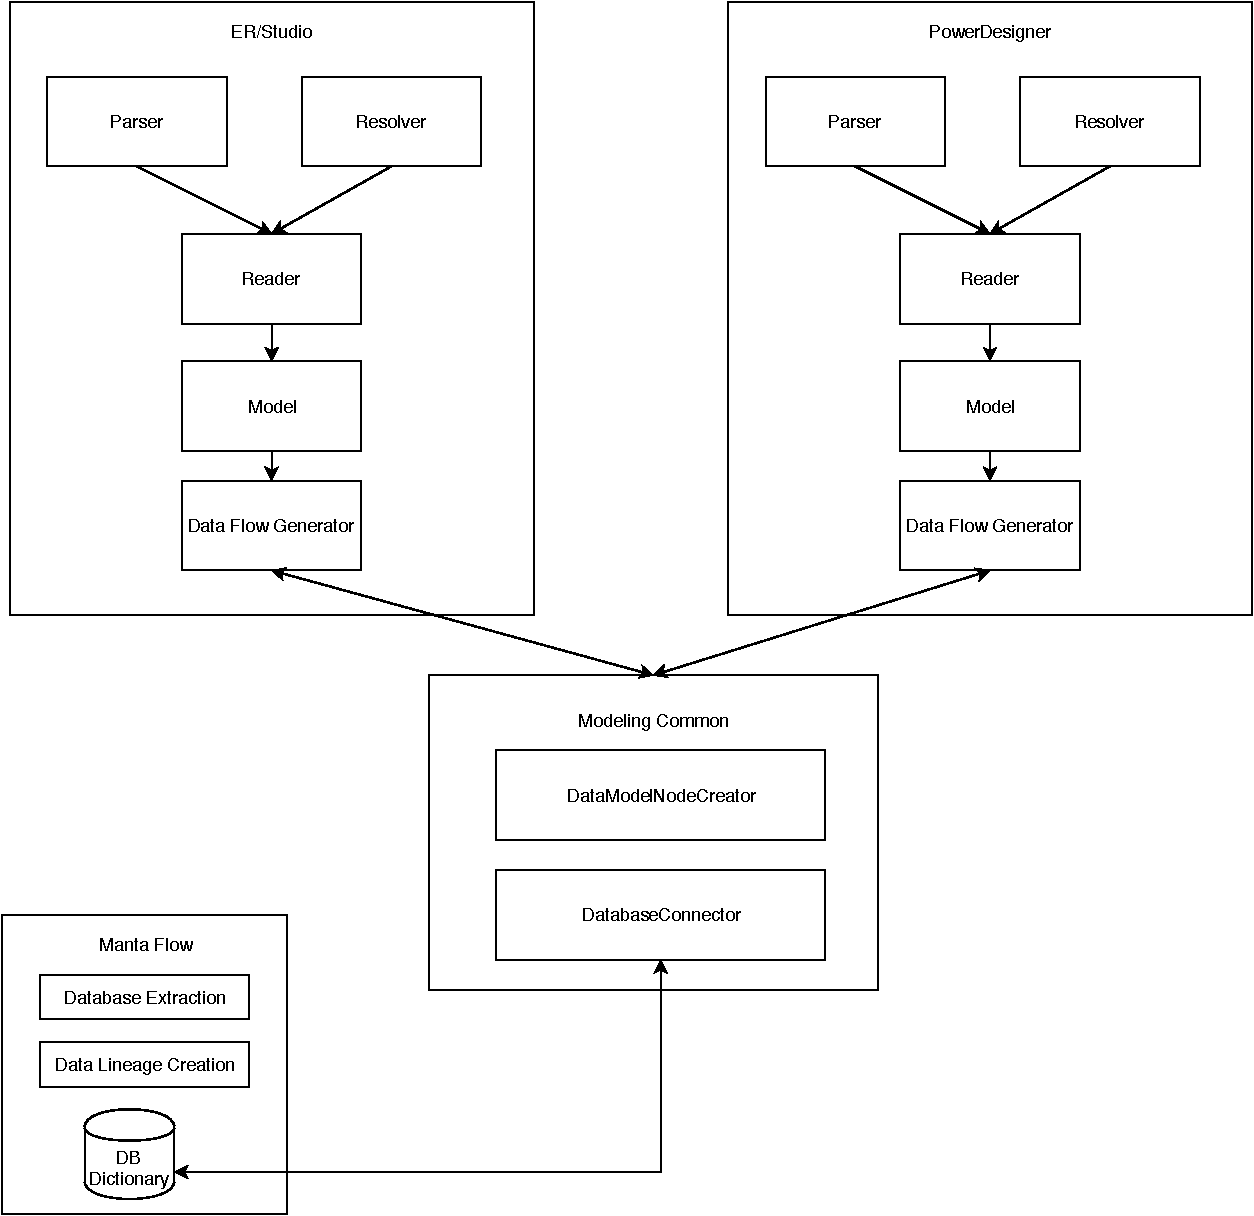
\includegraphics[height=14cm]{../img/SWArchitecture}
	\caption[Metadata Extractor Software Architecture]{A high level view on software architecture of Metadata Extractor}
	\label{SWArchitecture}
\end{figure}
\chapter{Implementation}

In this chapter we will mention the most important classes of our software and go through their main responsibilities. Here we describe the main three parts of the software - ER/Studio module, PowerDesigner module and the common part used by both of them. The shared module is a general artifact that is designed to be helpful when designing an extractor of metadata from an arbitrary modeling tool that is aimed to be included in Manta Flow. \\

We will go through the implementation from a higher perspective mentioning some classes and their methods from the source code of Metadata Extractor. 
Not every class and method will be described in this chapter, however precise programmer's documentation containing these information comes in a form of JavaDocs.

\section{ER/Studio}

\subsection{File Reverse-Engineering Tool}
\label{subsec:dm1_tool}

We introduced that file format that ER/Studio uses for storing data models consists of a relational databases like CSV tables (see \Cref{subsec:dm1_format}).
In order to be able to deconstruct objects stored in the files, we need to decrypt relations between tables in ER/Studio .DM1 files, as it is not easy to see how structured information is stored in those tables.
The task is to find out what links are leading between tables in the format. Relationships in this type of tabular data storage are done via primary and foreign keys. For this purpose we developed a little reverse engineering tools that should help us to reconstruct complex objects, as aspects of such objects are usually stored in multiple tables. \\

Input for this tool is an arbitrary .DM1 file and output must describe the logical layout. 
We observed the analogy of the file format logic with relational databases, which can be represented understandably by a relational diagram. Thus it would be nice  if output of the tool would be such diagram showing the organization of the .DM1 format.
However to create a diagram directly would be overkill we will use the knowledge that for creation of relational diagrams modeling tools are used.
The tools usually have the ability to transform some procedure defined in SQL into visual representation. 
For example based on the statement CREATE TABLE T modeling tool can draw a box in diagram representing table T. 
SQL surely can define columns of a table and create key constraints on columns as well. 
Modeling tools are able transform a foreign key column in table B that is a primary one in table A into a relationship between the two tables showed graphically in a diagram.

Thus, if we are able to generate a SQL create procedure for each of the tables from the file format and define by the query language primary and foreign keys of the SQL tables, modeling tools would transform such code into a visual representation of the analyzed file format.

To define a SQL create statement for the tables of ER/Studio's file format is straightforward once we parsed a .DM1 file. On the other hand deciding which column of a table is primary, which columns are foreign keys and to primary column of what table they refer to, is a more complicated task.
So we need to take the reverse-engineering process one step further - to be able to infer the keys.
Modeling tools commonly have the ability to reverse-engineer a relational database, however they are not able to tell relations between database tables. If so the knowledge is based on metadata from a database where keys are already defined, while the plain create statement in SQL do not provide any additional information like that.
In this situation we have no better option than to come up with own solution, as we have not found any utility inferring relations between tables solely based on column names or content of database tables.
Output of the reverse engineering tool therefore will be a SQL script containing table and key constraint definitions. 

As the development of the reverse-engineering utility is not the focal point of this work, the utility will not be an out-of-the-box general solution for deducing keys of relational databases, but should provide a basic overview of .DM1 files organization. 
Also it is not going to be a definitive foreign key deducing solution but is primarily concerned with the objects and properties picked by the analysis described above in \Cref{metadata_enumeration}.

In order to create the reverse-engineering utility we must decide what programming language we will write it in. Although there may be scripting languages that would make some operations, like joins on tables easier, we decided to use Java as Metadata Extractor itself is written in it and there is an important module - parser that the column deducing utility and Extractor, require. By developing both in Java it is suffices to write the parser once.\\

Firstly, an analyzed .DM1 file is parsed into a set of \classname{CsvTable}s.

When trying to find out what are columns with key constrained, the idea is to look at the loaded tables from two different views.

The first perspective is to take into account only metadata of a table. This approach is represented by the class \classname{DependencyCreator}. It treats columns that look like keys (eg. those which name ends with "ID", the policy is determined by \methodname{isOnBlacklist} method) as the same across all loaded tables. 
The main method here is \methodname{createDependencies} which pairs potential key columns and tables containing the candidate columns.
The class \classname{RelationFinderByTableDefinitions} allows querying over the structure found by \classname{DependecyCreator} showing what tables are possibly related through a series of joins.
Among others there is a general method \methodname{getDependenciesWithPaths} showing a sequence of joins needed to do in order to put put together records from table A with those from table B.

The second view takes into account data stored in the tables as well. 
When analyzing what are relations between columns, we consider a table as a collection of columns. A \classname{CsvColumn} stores a set of values from all records of its table at position of the column. 
This way we can examine if columns with same names have similar contents.
In contrast when getting records from a table we see it as a collection of \classname{CsvRow}s.
The \classname{RelationFinderByTableContents} class is used for the further search for key columns.

It filters tables that have no content, thus are irrelevant for this approach.
The relation finder class which is analyzing contents of tables has a method for determining if a column can be considered a primary key of a table.  That is true only if a columns contains solely distinct values as a primary key must be completely unique in a table.
The relation finder also has a method finding out if a column can possibly be storing foreign keys. If column A contains foreign keys of primary keys specified in column B, each entry of A must be present in B, thus A must be subset of B.
In .DM1 file format there is a table \classname{Identity Value} that explicitly pairs tables with their primary key columns. Of this information the reverse engineering tool takes advantage as well.
The class also inspects if the primary keys are defined in strict order or if there is some pattern in how primary keys are listed in a .DM1 table.

The classes above allowed us to look from multiple perspectives at metadata and data of tables in the analyzed file format.
To put it all together and to finally generate the desired output in form of a SQL code defining .DM1 tables and their keys out of the analysis done the class \classname{TablesToSQLConverter} is used.
The main method is \methodname{writeMySQLSource} which at the beginning defines SQL create statement for each table from ER/Studio source file. 
Then the phase of creating the key constraints takes place. It operates on candidate columns that satisfy policies in \classname{DepedencyCreator} to be key columns and are present in at least one table so one or more joins can be made using the keys.
There is also space for defining manually the knowledge we gained by inspecting the format using \classname{RelationFinder*} classes by inserting pairs table and its primary key.
At first place primary keys defined from user-defined information are set, then the information stored in \classname{Identity Value} table is used for key definition. Lastly, key inference based on policies a name of a column in context of its table takes place. For example if a table is called tableA\textunderscore id it is very likely it is a primary key if it comes from table called tableA.
If a column is set as a primary key in one table for each of the remaining tables that contains the column with same name, the column is marked as a foreign key.
In the case there are columns that were chosen as candidates for being keys but no constraint was assigned to them in previous steps, in one of the tables which contain such column is marked as a primary and in the rest as a foreign one. That may cause slight inaccuracies in the final result, but the main message should not get lost.

\subsection{Parser}
\label{subsec:dm1_parser}

We already discussed in \Cref{subsec:dm1_format} that the files storing objects we want to recreate from ER/Studio are using format, which is basically a sequence of CSV tables. In order to be able to further process the information saved in the file format, we need to load the contents of those tables into corresponding data structures. That is what parsers are for.

Already existing CSV parsers are made to process a single CSV table per file. There is no unified definition for the comma-separated-value files, but usually they do not allow naming CSV tables as present in .DM1 files.
What is important to say about CSV record is, that each entry is located on a separate line, fields in an entry are separated by a comma, the last record is followed by line break. A field may contain a comma or line break but must be enclosed by double quotes.
If a double quote appears in a field, it must be in the enclosed section and the quote itself must be doubled \cite{RfcCSV}.

The structure we need to parse contains tables consists of a name on a single line, definition of columns and entries. Two tables are separated by a single empty line.

Putting it all together it seemed to be easier to develop our own parser for .DM1 files that processes the files into a set of tables identified by their names.

A single table is represented by an instance of the class \classname{CsvTable} which contains its name, definition of columns, in other words names for each of its properties \classname{CsvColumnDefinition}, and finally records themselves - instances of \classname{CsvColumn} which are contents of a table.

However, the view on a table may vary by usage of the parser. Using the reverse-engineering tool, we inspected what values are stored in a column, examined the domain of values across all records etc. 
On the other hand, if we see a table as records, each record having properties, one property is one column, from this perspective a table is a set of rows.
The second case is needed when reading the contents of a table for the sake of obtaining its records.

Getting a name of a table is an easy job as its just a single textual line. To resolve a record, get the individual fields separated by a comma, correctly is a slightly more challenging task, since the rules described at the beginning of the chapter must be taken into account. 
We designed an automaton that accepts well formed records of our CSV table.

We propose a non-deterministic finite automaton, even though it can be translated to a deterministic one, we consider an NFA to be more clear and descriptive in this situation.
Set of states is $Q = \left\{i, q, e, a, f\right\}$.
Alphabet $\Sigma$ is a set of chars that can appear in a string, since that is what the automaton processes, together with $\lambda$ - an empty string.
I is the initial state.
Transitions are illustrated in the following Figure 5.1.

\begin{figure}[H]
\begin{center}
	\begin{tikzpicture}[scale=0.2]
	\tikzstyle{every node}+=[inner sep=0pt]
	\draw [black] (40.8,-21.4) circle (3);
	\draw (40.8,-21.4) node {$i$};
	\draw [black] (71.5,-33.2) circle (3);
	\draw (71.5,-33.2) node {$f$};
	\draw [black] (71.5,-33.2) circle (2.4);
	\draw [black] (21.1,-33.2) circle (3);
	\draw (21.1,-33.2) node {$q$};
	\draw [black] (48.2,-33.2) circle (3);
	\draw (48.2,-33.2) node {$a$};
	\draw [black] (39.9,-45.7) circle (3);
	\draw (39.9,-45.7) node {$e$};
	\draw [black] (40.8,-15.4) -- (40.8,-18.4);
	\fill [black] (40.8,-18.4) -- (41.3,-17.6) -- (40.3,-17.6);
	\draw [black] (37.813,-21.495) arc (299.55605:11.55605:2.25);
	\fill [black] (38.91,-19.09) -- (38.95,-18.14) -- (38.08,-18.64);
	\draw (33.93,-17.59) node [left] {$Q\setminus\left\{",\backslash,\right\}$};
	\draw [black] (43.6,-22.48) -- (68.7,-32.12);
	\fill [black] (68.7,-32.12) -- (68.13,-31.37) -- (67.77,-32.3);
	\draw (54.94,-27.83) node [below] {$\backslash n$};
	\draw [black] (38.23,-22.94) -- (23.67,-31.66);
	\fill [black] (23.67,-31.66) -- (24.62,-31.68) -- (24.1,-30.82);
	\draw (30.04,-26.8) node [above] {$"$};
	\draw [black] (18.622,-34.87) arc (-28.28273:-316.28273:2.25);
	\fill [black] (18.27,-32.25) -- (17.8,-31.43) -- (17.33,-32.31);
	\draw (13.73,-34.26) node [left] {$Q\setminus\left\{"\right\}$};
	\draw (39.91,-33.56) node [left] {$Q\setminus\left\{,\right\}$};
	\draw [black] (23.6,-34.86) -- (37.4,-44.04);
	\fill [black] (37.4,-44.04) -- (37.01,-43.18) -- (36.46,-44.01);
	\draw (29.59,-39.95) node [below] {$"$};
	\draw [black] (42.69,-44.6) -- (68.71,-34.3);
	\fill [black] (68.71,-34.3) -- (67.78,-34.13) -- (68.15,-35.06);
	\draw (56.92,-39.97) node [below] {$\backslash n$};
	\draw [black] (41.56,-43.2) -- (46.54,-35.7);
	\fill [black] (46.54,-35.7) -- (45.68,-36.09) -- (46.51,-36.64);
	\draw (44.66,-40.78) node [right] {$,$};
	\draw [black] (37.4,-44.04) -- (23.6,-34.86);
	\fill [black] (23.6,-34.86) -- (23.99,-35.72) -- (24.54,-34.89);
	\draw (31.41,-38.95) node [above] {$"$};
	\draw [black] (40.01,-42.7) -- (40.69,-24.4);
	\fill [black] (40.69,-24.4) -- (40.16,-25.18) -- (41.16,-25.22);
	\draw [black] (46.61,-30.66) -- (42.39,-23.94);
	\fill [black] (42.39,-23.94) -- (42.4,-24.88) -- (43.24,-24.35);
	\fill [black] (46.61,-30.66) -- (46.6,-29.72) -- (45.76,-30.25);
	\draw (45.13,-26.01) node [right] {$\lambda$};
	\draw (43.87,-28.59) node [left] {$,$};
	\end{tikzpicture}
\end{center}
\caption[NFA Accepting a CSV Line]{Non deterministic finite automaton accepting a line of a CSV table in .DM1 file. In the state $a$ and $f$, the end of a CSV field is recognized and accepted.}
\end{figure}

When parsing a CSV record consisting of multiple fields not only we want to determine the end of a CSV entry but to collect the fields as well. That is what the, at first sight redundant, state A expresses. Once the automaton gets to the state $a$, the end of a field in the input is indicated. The boundary of the last field of an entry is, however, recognized in the accepting state $f$.

The parser's interface is a single method \methodname{readFile} taking a file to process and returning pairs of table name and an instance of \classname{CSVTable}.

\subsection{Model}

The purpose of the model component is to provide an access for reading to both a raw structure of a processed source file and a fully loaded hierarchy of objects we reconstructed from a file.

The crucial objects and the important properties of theirs result from the analysis of ER/Studio data models listed in \Cref{metadata_enumeration}. Those are the ones the model is required to capture.

The perspective of a raw file structure loaded to memory is represented by an interface \classname{ErStudioFile} where either all tables from file can be retrieved via \methodname{getAllCsvTables} or a single table by its name using the \methodname{getCsvTable} method.

An ER/Studio solution - a set containing one logical data model and arbitrary number of physical models implements \classname{ErStudioSolution} interface. All the objects contained in the data models stored in such solution can be retrieved using the interface's methods. A solution is defined in a file, the relative name of the file where the solution is an internal one is returned when called \methodname{getFileName}.

Since a .DM1 file is not restricted to storing a single solution, but may reference external models as well, thus there may be objects from multiple solutions saved in a file. If name of the solution's origin file is identical with the name of .DM1 file from which it was loaded, it is an internal file. The overall structure of a file is represented by \classname{ErStudioFileModel} that has a main solution - the internal one and possibly references external solutions.

A base behavior of both logical and physical data models is defined in \classname{DataModel}.
A data model has a name and contains owners. An instance fulfilling \classname{DataModel} interface must have property of type \classname{AbstractionLayer} set to either \methodname{Logical} or \methodname{Physical} just like every object that is contained in a model.

\classname{PhysicalDataModel} has an important addition, that it can tell the database platform the low-level model is designed for. In enum class \classname{Platform} all the database management systems ER/Studio supports are captured with an extra entry for an unknown DBMS.

\classname{Owner} is either \methodname{Logical} or \methodname{Physical} according to what objects it can own and what type of model it may belong to. 
It has name and allows access to the objects owned by it.

The objects that can be mapped to another object implement interface \classname{Mappable<T>} where the type parameter defines what is the kind of the mapped counterpart.

Objects in a data model that can be described further by definition and note while having a name can fit into \classname{DataObject} interface. These can be either \classname{CompositeDataObject} or \classname{SimpleDataObject}.

An interface for the composite ones describes what is expected from a table or an entity.
They have the very same properties that is why a single class is enough to capture their structure. Which of the two it is is decided by \classname{AbstractionLayer}.
The composite one can be mapped to another \classname{CompositeDataObject} and may contain simple objects.

The \classname{SimpleDataObject} class is used to represent columns or attributes. Equivalently, layer of abstraction is crucial to determine whether the object fulfilling the interface can be stored in \classname{PhysicalDataModel} or \classname{LogicalDataModel}. It must be invariant, that the whole subtree of objects, beginning in a data model must have the same abstraction layer defined.

The reason to represent pairs of, at first sight, different concepts of tables-entities and columns-attributes in a single classes is based on how ER/Studio treats them internally. Given that columns and attributes are stored in a single CSV table and the distinction if such object is of one or another type, is made based only on the fact to which data model, physical or logical, it belongs to. The two types have the very same set of possible attributes. This can be applied to composite objects as well. Even data models are treated similarly, only there is an additional attribute related to DBMS type in the case of physical models, while the logical ones do not need such information.
 
\TODO{class diagrams?}
\subsection{Resolver}

The purpose of the resolver unit is to actually create the objects which are form data models which Metadata Extractor obtains from modeling tools. These results of the resolver module, thus are fulfilling the contracts specified by the functionality defined in the model.

Outline of what the resolver module does is that it via \classname{ErStudioFileModelBuilder} creates the whole structure representing an input .DM1 file as instance of \classname{ErStudioFileModel}. It builds an internal solution, then external solutions are created and at the end resolving of mappings that lead across the solution using \classname{ExternalMapper} takes place.

Typically, for each interface, we will create an implementation. In Java it is common to call the classes fulfilling an contract \classname{*Impl} where * is a placeholder for the name of an interface. We stick to this naming convention. 
The \classname{*Impl} classes, in contrast to the interfaces that are used to describe the model component, need to dispose of methods for setting up and adding properties or substructures as the model's reading methods would not be very meaningful otherwise. These classes can be found in the imp package. \\

We defined what is expected from the classes and added the functionality helping to set up the objects, once we gathered required information.
So the last missing piece of puzzle needed to create the objects is how to gather the required information.
The logic taking care of collecting the needed data is hidden in the package builder.
The skeleton of how an instance of \classname{ErStudioSolution} is created is prescribed in the \classname{AbstractDataObjectsBuilder}'s method \methodname{buildErStudioModel} that follows the paradigm of the template method design pattern and defines the steps needed to take in order to construct an instance of \classname{ErStudioSolution} solution, no matter if it is of internal or external type.
The template method enforces a tree of objects in a solution is build from the top down.
The very first is to step is to create a root of such tree - an instance of \classname{ErStudioSolution} that is being build, then \classname{DataModel}s from the solution are loaded, \classname{Owner}s follow, \classname{CompositeObject}s after and finally \classname{SimpleObject}s. 
Child instances are appended to their parents just when created.
The abstract builder contains common methods for construction of objects. Those methods are not dependent on representation, only require a set of properties as input to be able to attach them to resulting objects to make them complete. The groups of properties needed to be collected about each type to proceed the construction are described by interfaces in the package modeledobjectproperties.

The specific way of gathering the information about objects to be reconstructed is tied with details of how the objects are saved in the file format. Concrete builders 	\classname{InternalDataObjectsBuilder} along with \classname{ExternalDataObjectsBuilder} provide implementation to the abstract methods.
In the case of internal solution, information about objects are retrieved from CSV tables, where for each table there is a dedicated and references across the tables are resolved.
On the other hand, in case of external solutions, they are fully represented in a single CSV table that stores XML structures describing these objects. The implementations of the placeholders in \classname{ExternalDataObjectsBuilder} uses a simple SAX XML parser to retrieve the desired data described in modeledobjectproperties.

\classname{InternalDataObjectsBuilder} has one more responsibility and that is to create mappings between \classname{Mappable} objects in a solution with a help of \classname{InternalMapper}. 

The  \classname{InternalMapper} class only has knowledge about the layout of a CSV table containing internal mappings, just like the \classname{ExternalMapper}, that we will need later, has about the definitions of external mappings. However the logic of putting objects to maps-to relation is coded in the \classname{AbstractMapper} class.
It goes through a table which definition fulfills the interface \classname{MappingTable} and links pairs listed in the table by mapping, if their types are equivalent.

\TODO{a class diagram?}

\subsection{Reader}

The reader component puts together the parser module with resolver and produces a data structure by what the model component defined. \\

\classname{ErStudioDm1Reader} crawls through directory with input .DM1 files processing them. Each time the \methodname{read} method is called the parser processes next file from the input folder. Parser's product is handed to resolver resulting in \classname{ErStudioFileModel} that is what \methodname{read} returns.

\subsection{Data Flow Generator}

Having constructed the objects defined in the model unit, Metadata Extractor sends them to Data Flow Generator unit, where the model get transformed into an output graph and connects to Manta Flow to enrich the graph of ER/Studio objects by data lineage.

Before describing the workflow of the generator unit, let us mention its layout.
There is a scenario that executes independent tasks. A task is a routine that has an input and an output. In out case we will use a single task whose input will be a data structure described by the model unit and output a graph with extracted information.

 Namely, \classname{ErStudioDataflowScenario} reads an input file, and executes the task - \classname{ErStudioDataflowTask}. 
 
 The method which tasks must override and gets called is the \methodname{doExecute}. In this particular task it is needed to go through the whole hierarchy of the input data structure - \classname{ErStudioFileModel} unroll solutions - internal as well as external.

A suitable \classname{Connection} corresponding to a physical data model is made of information from a data model and .ini file to be able to pair physical data model objects with those from database dictionaries.

Once assigned the connections to physical models, we can traverse the data models trees, creating nodes using \classname{DatabaseConnector} in the case of physical level, whereas when it comes to logical objects Metadata Extractor takes advantage of \classname{DataModelNodeCreator}.

As the tool creates the mappings symmetrically, the full information is captured on both levels. This way, it is possible to create all the mapping edges by going through all objects from a single level of abstraction, no matter which level though as each mapping edge is contained in both of the levels.
For the sake of simplicity, as there usually is less logical models generally a logical model contains fewer objects than a physical one, data flow generator goes through all the logical objects, creating their node representation and collects the attributes, that have to be linked to a column.
Then physical objects are created as nodes and if the just constructed node has a mapping, MAPS\textunderscore TO edge is set between the mapped nodes.


\section{PowerDesigner}

\subsection{Parser}

The files storing the data model objects we want to reconstruct from PowerDesigner are of XML type.
In the analysis section we already discussed the possibilities when it comes to reading XML files. We concluded that the most suitable approach in our case should be loading the inputs to a DOM tree data structure.
We did not try to reinvent a wheel as there is many DOM parsing services. 
Given that in the ecosystem of Manta software there is an internal artifact made for transforming XML to DOM Metadata Extractor will make use of it.

\subsection{Model}

Let's start describing the main structure the model has to capture generally.
In the case of PowerDesigner a model is saved in a single file. 
Thus \classname{DataModel} has the name of the file where it is stored and its sub objects, then the hierarchy goes like this \classname{Schema} has \classname{CompositeObject}s which contain \classname{SimpleObject}.
This basic skeleton of a tree structure is present in each of the three data models. What more, on logical and conceptual level, as they are represented by an EER diagram, an entity can inherit from another one, thus an interface \classname{Entity} introducing the concept of parent entity will be used by them. Each of actors may have some metadata providing further description and extends the interface of \classname{NamedObject}.
These interfaces are generic and provide the common structure.
For every model type there exists a package, where specific objects' contracts lies. These concrete interfaces on one hand takes over the common concepts. On the other hand may be easily extended if a new functionality, which is data model specific, is identified.

\classname{Mappable} interface is present to be realized on instances of \classname{CompositeObject} or  \classname{SimpleObject}, however a target of a mapping is a globally unique id of an element, not another instance directly. Since by the nature of mappings in PowerDesigner the actual representation may be unreachable yet.

\subsection{Resolver}

The impl package contains the implementational counterpart to the model unit.
Common concepts with no that do not take part in data models in reality and are present to minimize redundancy and provide way to handle similar objects, for example \classname{CompositeObject}, are implemented as abstract classes - their names are prefixed Abstract. The actual objects that are implemented via *Impl classes.

The construction logic of a data model is concentrated in the build sub package.

The API for creating a data structure representing a data model is simply defined by \classname{DataModelBuilder} on what the method \methodname{buildDataModel} may be called and the result is collected from \methodname{getResult} operation.

However, there is a different strategy used for each of the data models based on type it is. So when processing a PowerDesigner file the program must determine the suitable implementation of \classname{DataModelBuilder} accordingly. 
A factory template class \classname{BuilderFactory} is used to determine which implementation - \classname{PhysicalDataModelBuilder} or \classname{LogicalDataModelBuilder} or \classname{ConceptualDataModelBuilder} by the extension of the processed file.

The outline how the builders work is proposed in the \classname{AbstractDataModelBuilder}. Also the functionality independent of type of a specific data model is written here, the way to do it is to look on objects from the perspective of abstract classes providing the general features.

The implementations take an advantage of the fact that forming a tree like structure from an XML format is natural and straightforward, that is why for now we will omit a general point of view on a construction data model that would hide the convenience and context provided straightforwardly by DOM nodes. 
Requests for specific DOM nodes in the builders are done using XPath, which allows querying fully loaded XML trees.

\subsection{Reader}

The reader unit formed by \classname{PowerDesignerXmlComponentReader} reads a directory containing output file of PowerDesigner that are at the same time inputs for Metadata Extractor - .pdm, .ldm or .cdm files and identifies related groups of them. Then proceeds one group after another, in parsing the XML files into a DOM document and passing the DOM trees to resolver that creates a corresponding set of \classname{DataModel} objects using resolver's \classname{DataModelBuilder}, which can be further passed to the data flow generator unit.
 
Input directory containing file to process is the input for \classname{PowerDesignerXmlComponentReader}. The reader recursively discovers the directory and collects the file that will have to be resolved using the \methodname{collectFiles} method. When a data model file is found, its dependencies are checked using a \classname{SAXParser} and a simple handler \classname{TargetSAXHandler} created for the purpose of getting paths to related models from an XML. The found files, however must be in the input directory, so if it is not the case, the reader tries to resolve their paths and check if there is no file with matching sub path within the input directory. If it is a bidirectional edge between the files is created. 
Once all the files from input are collected component creation takes place so the input set is split into smaller logically connected groups.

Then when the main API method of a reader, the \methodname{read} method, is called, it returns one processed component - a set of related reconstructed \classname{DataModel}s. 
That means the reading method is stateful and \methodname{canRead} checks if there are any component left to be returned.

\subsection{Data Flow Generator}

When translating a component of reconstructed data models, a suitable \classname{GraphBuilder} must be chosen based on the layer of abstraction for each data model using \classname{GraphBuilderFactory}.
Then the tree of data model objects is traversed. When dealing with physical data model, \classname{PhysicalGraphBuilder} is used, underlying \classname{DatabaseConnector} searches for the modeled database objects. A suitable \classname{Connection} corresponding to a physical data model is made of information from a data model and .ini file, loading connection details from .dsn and .dcp files is not supported yet.
On the other hand, physical and logical data models use the generic \classname{ModeledGraphBuilder} for creating nodes representing objects brought from data models of greater abstraction.
The generator collects nodes that have mappings by their ids and once all the data models in the processed components are fully built, it means we can resolve the mapping as there are both ends of the MAPS\textunderscore TO type edge we need to create them. Then we simply look at to what ids are objects mapped, obtain an actual representation of these ids put them into the relation by creating the edge.

\section{Extensibility}

For the sake of extracting metadata from modeling tools we developed a unit where a component for a specific tool meets manta flow.
The artifact where the common bridging logic is stored is called manta-dataflow-generator-modeling-common.
Physical data models need to be paired with corresponding connections to DBMS in order to correctly pair the same database objects that appear both in a physical model and in a database dictionary extracted by Manta Flow. This functionality is provided by implementations of interface \classname{DatabaseConnector}. Details about the target database of the low-level data model are kept in \classname{Connection}. The API to database dictionaries created by Manta is provided by \classname{DataflowQueryService}. 
Having collected information of a physical object, either a column or a table, the query service tries to find it in the dictionaries using \methodname{createColumnNode} or \methodname{createTableNode}. 
If the service succeeds, matched node from a dictionary is appended to the output graph, otherwise null is returned from a create method and our tools copes with the situation in such a way, that it creates a node that has no backing in a live database, marking the node's attribute source type to MODEL to make clear in the output, that it is an artificial node based only on a physical data model. It can be from two reasons - the database object does not exists or we provided inaccurate/incomplete data to identify it.

So the first general requirement for a general extractor from data modeling tools is to be able to organize extracted metadata in such a way that \classname{DatabaseConnector} may be called and ideally match the modeled objects with the extracted ones.
This is a very important step as this pairing is the prerequisite for business data lineage creation. If the physical modeled object do not match the ones from database that take part in data lineage, there is no flow to be propagate to higher levels of abstraction via maps to edges and the result of interpolation will be an empty set of edges.

Secondly, we have defined a common way of creating nodes representing objects extracted from data models of higher abstraction than the physical ones - conceptual and logical.
We define a set of methods where each is responsible for creation of node representation of a type of object that may appear in the data models. Most commonly a modeling tool will support only subset of the types the node creator is able to construct. However that is not a problem as the hierarchy is not strict and it can be built to be compliant with concepts of a specific modeling tool. 
For example it is not necessary to build an attribute under an entity node if a modeling tool does not allow such concept, just like an owner node is not necessary as there is no strict rule if the tools should support it or not.

We have discussed the modeled objects on conceptual and logical level are described by ER or EER diagrams. 
The important fact is that the possible kinds of objects will be the same in both models, that is why a single interface \classname{DataModelNodeCreator} for high-level node creation may be used.
However it must be implemented by two different classes \classname{LogicalDataModelNodeCreatorImpl} and \classname{ConceptualDataModelNodeCreatorImpl}, so details about node's type can be specified, therefore the nodes will not mix between the layers.
\classname{Resource} differentiates technologies, in our case it makes sure objects extracted from modeling tools are aggregated by what specific tool is their origin.

To attach metadata about a node, such as its definition or a comment, object that is being transformed into node representation has to implement interface \classname{NodeMetadata}.
The contract forces the implementers to expose the metadata to be attached to node representing them in the output in form of strings. 
More precisely, the objects have to fill a \classname{Map<String, String>} data structure where a key is the name of a property. 
These metadata are shown when presenting the output graph and further describe the extracted objects. \\ 

Basically, the outline when implementing a metadata extraction from a different modeling tool is the following:

\begin{enumerate}
	\item Define the crucial data model objects, relations between them, hierarchy and properties interesting enough to be captured in data lineage by read-only interfaces. That is model component. 
	The objects that will be represented as standalone nodes in data lineage visualization at the end have to implement \classname{NodeMetadata} interface.
	\item Depending where from the data models are obtained, this phase generally retrieves data models from a storage. It may be by calling a web API to get data mode objects from a server, retrieving them from a database, or like in the case of Metadata Extractor, by parsing a file.
	\item Resolving takes place once some representation of data models was reached. This stage transforms the acquired object into objects conforming aspects described by the model module.
	\item Data flow is generated from the output of the resolver. This module translates data structures describing modeled objects to graph nodes. 
	Database objects from physical data models are expected match the ones in database dictionaries of Manta that were extracted directly from databases. 
	The communication with Manta is done via \classname{DatabaseConnector} and \classname{Connection} that is assigned to a physical model.
	Logical and physical modeled objects are transformed to node representation using corresponding implementation of \classname{DataModelNodeCreator} - logical and physical respectively.
	Once the nodes are created out of the extracted objects, resolving of mappings between the layers takes place.
	Linking correctly physical nodes, that were paired with the ones from database dictionary, with higher level nodes is crucial to bring business lineage. 
	However there is no strict skeleton for this process as the approaches to how modeling tool realizes mapping across data models may be substantially different, as we have seen in case of PowerDesigner and ER/Studio.
\end{enumerate} 

\section{Technologies}

The quality of programmer's toolbox may have a huge influence on his productivity when developing a more complex piece of software.

\begin{itemize}
	\item Java 8 \\
	To be able to integrate Metadata Extractor into the ecosystem of Manta Flow the best solution is to use Java as the APIs of the data lineage software are written in this programming language.
	\item Maven \\ 
	For dependency management, the most usual tool when programming in Java is used - Maven. In order to build the program, all the Manta Flow artifacts which Metadata Extractor depends on must be obtained successfully. However those artifacts are reachable only within Manta's private network.
	\item Spring \\
	For program configuration, inversion of control via Spring's XML files is used. Along with .properties, where variables used in the spring files may be (re)defined.
	\item JUnit 4 \\ 
	The standard for unit testing Java programs is the JUnit framework we use.
\end{itemize}

\section{Testing}

Automated unit tests validating the crucial parts of the implementation are a huge help to determine correctness of Metadata Extractor's logic.

\subsubsection{ER/Studio Parser}

The correctness of parsing process is checked by class \classname{ErStudioFileFormatParserTest} which is controlling how many CSV tables from a parsed .DM1 files was obtained. Given that the format consists of a constant number of tables if the count is mismatching it indicates a flaw in detecting borders of tables.
Also every CSVs should be valid in the way that each row in a table must have the same number of fields. If it has not, we assume there is problem on our side and parser does not pass the tests.

\subsubsection{Reader \& Resolver}

Testing of the output of the reader module shows tells a lot about the resolver's correctness, since the logic of reader is actually provided by this module. 
From the nature of reader, that it connects resolver and parser, these tests rely on the fact that resolver works correctly and we assume this is true as far as the parser module tests are passing.
The goal of the reader tests is to find out whether all objects from data models were successfully loaded into data structures described by the model module.
In case of ER/Studio the testing compares expected statistics about data models such as number of physical models in a solution, entity count of logical model etc. with the amount of objects that were loaded actually by reader.
Secondly, some specific objects from hierarchy of a data model that is on input are picked and checked if they were loaded accordingly. Tests check metadata of those objects and mappings with another objects as well. \\ 

PowerDesigner must create components correctly, so is present a test for checking if number of components is correct.
The main reader test consists of reading file by file, thus size of a component is one every time (the components creation correctness is ensured the previous test).
The expected values and objects are loaded from JSON sources file where they are stored in a deserialized form.

\subsubsection{Data Flow Generator}

In data flow generator, we are interested if objects loaded by reader are transformed into nodes as expected.
The skeleton is similar for both modeling tools. \\

\classname{*GraphBuilderTest} classes are testing independently drawing of each of the layers. The graph created by the \classname{*GraphBuilder} classes can be saved as a .txt file describing the graph. 
For each test we have an expected output of how a correct output graph should look like. The two files are compared, if they are same the behavior of the output building process is correct.

The previous test checked the representation of the layers independently, in \classname{*DataflowTaskTest} all layers from a solution, or from a component when talking about PowerDesigner, are constructed with mapping edges leading between them. Outputting graph is also serialized to a textual file. Next, mapping edges are filtered from the file and compared with expected set of maps\textunderscore to edges. 




\chapter*{Conclusion}
We have developed a piece of software capable of extracting metadata from two data modeling tools - SAP PowerDesigner and ER/Studio Data Architect. To achieve this a thorough analysis was required to identify relevant features of the tools, as well as studying the way data models are represented in memory. 
A framework bridging Manta Flow with objects extracted from data models was developed, therefore further support of another modeling tools may take advantage of it and can be aware of what contract to meet in order to create business lineage and to enrich the physical one.

One of our aims was to explore possibilities of modeling data lineage in modeling tools.
We went through it and described the important aspects of the lineage and compared it to the one that Manta Flow creates. 
Initially, there was an idea, that if a tool allows the functionality, it would be nice to compare the actual lineage, physical or business, computed by Manta Flow and Metadata Extractor, with the modeled one. 
However, the modeling tools we analyzed do not provide any API, that would allow us to correct or compare the flows specified in the tools. 
An option would be to try to manually adjust the lineage, but this approach would be not easy and fragile at the same time.

\addcontentsline{toc}{chapter}{Conclusion}


%%% Bibliography
%%% Bibliography (literature used as a source)
%%%
%%% We employ bibTeX to construct the bibliography. It processes
%%% citations in the text (e.g., the \cite{...} macro) and looks up
%%% relevant entries in the bibliography.bib file.
%%%
%%% The \bibliographystyle command selects, which style will be used
%%% for references from the text. The argument in curly brackets is
%%% the name of the corresponding style file (*.bst). Both styles
%%% mentioned in this template are included in LaTeX distributions.

\bibliographystyle{plainnat}    %% Author (year)
% \bibliographystyle{unsrt}     %% [number]

\renewcommand{\bibname}{Bibliography}

%%% Generate the bibliography. Beware that if you cited no works,
%%% the empty list will be omitted completely.

\bibliography{bibliography}

%%% If case you prefer to write the bibliography manually (without bibTeX),
%%% you can use the following. Please follow the ISO 690 standard and
%%% citation conventions of your field of research.

% \begin{thebibliography}{99}
%
% \bibitem{lamport94}
%   {\sc Lamport,} Leslie.
%   \emph{\LaTeX: A Document Preparation System}.
%   2nd edition.
%   Massachusetts: Addison Wesley, 1994.
%   ISBN 0-201-52983-1.
%
% \end{thebibliography}


%%% Figures used in the thesis (consider if this is needed)
\listoffigures

%%% Tables used in the thesis (consider if this is needed)
%%% In mathematical theses, it could be better to move the list of tables to the beginning of the thesis.
\listoftables

%%% Abbreviations used in the thesis, if any, including their explanation
%%% In mathematical theses, it could be better to move the list of abbreviations to the beginning of the thesis.
\chapwithtoc{List of Abbreviations}

ER \tab Entity-Relationship \\ 
EER \tab Enhanced-entity-Relationship \\
CDM \tab Conceptual Data Model \\
LDM \tab Logical Data Model \\
PDM \tab Physical Data Model \\


%%% Attachments to the bachelor thesis, if any. Each attachment must be
%%% referred to at least once from the text of the thesis. Attachments
%%% are numbered.
%%%
%%% The printed version should preferably contain attachments, which can be
%%% read (additional tables and charts, supplementary text, examples of
%%% program output, etc.). The electronic version is more suited for attachments
%%% which will likely be used in an electronic form rather than read (program
%%% source code, data files, interactive charts, etc.). Electronic attachments
%%% should be uploaded to SIS and optionally also included in the thesis on a~CD/DVD.
%%% Allowed file formats are specified in provision of the rector no. 72/2017.
\appendix
\chapter{Attachments}

\section{Building}
\label{build}

The build process is ensured through Maven with dependencies specified with its pom.xml files.
However, in order to build Metadata Extractor "secret" dependencies owned by MANTA are needed. Otherwise the project will not compile successfully. 
Also in order to gain the whole functionality of our tool a context provided by Manta Flow's database extractors, post processing done on server, where the interpolation takes place, and visualization of data lineage which is also part of the server's functionality is needed. 
There is a command line user interface putting all the parts together and must be backed by manta server with graph database that is running user interface as well. The crucial parts of Manta Flow though can not be built without having access to MANTA's code repository.

Even with the access to the repository, MANTA is a proprietary software and running its products requires a valid license.

Thus only those jar files that are needed for running tests are attached. They cannot be rebuilt by a user.


\section{User Documentation}

To run Metadata Extractor the prerequisite is to have Java 8 on a computer. \\

As we mentioned in \Cref{build} with this work come attached only files needed to demonstrate functionality on tests due to licensing of Manta Flow product

\subsection{Tutorials}

\TODO{to include or not}

\section{Cooperation with Manta Flow}

In the case a user has access to Manta Flow server and command line interface (CLI) with corresponding licenses, the full functionality of Metadata Extractor can be manifested.

The CLI has an aggregate input directory, further divided by technologies.
Subdirectories erstudio and powerdesigner are located in input.  
Both have the same following layout: 
It contains systems, a system is logical group of modeling files to be processed.
System consists of two items - one is containing the models from which metadata will get extracted and a .ini file where connection specifications to physical models are defined.

The systems to be processed from input are specified by .properties file   /scenarios/etc. 
For each system in input a property file specifying a name of the system folder to be processed must be present. \\ 

To proceed the extraction user runs one of the executable files provided \textunderscore run.sh for Unix-like, \textunderscore run.bat for Windows machines respectively.

\section{Full List of Modeling Tools Metadata}
\label{full_list_metadata}

\subsubsection{Conceptual \& Logical Data Model}

\subsubsection{ER/Studio}

\subsubsection{CDM}

ER/Studio does not support conceptual data models.

\subsubsection{LDM}

\begin{itemize}
	\item Owner
	\item Entity 
	\begin{itemize}
		\item Name 
		\item Attributes 
		\item Definition
		\item Note
		\item Where Used
		\item User-Defined Mappings
		\item Owner
		\subsubsection{Properties We Will Not Extract}
		\item Permissions 
		\item Keys 
		\item Relationships 
		\item Constraints 
		\item Naming Standards 
		\item Data Lineage
		\item Security Information
		\item Attachment Bindings
	\end{itemize}
	\item Attribute
	\begin{itemize}
		\item Name
		\item Definition
		\item Notes
		\item Where Used
		\item User-Defined Mappings
		\subsubsection{Properties We Will Not Extract}
		\item Datatype
		\item Default
		\item Rule/Constraint
		\item Reference Values
		\item Naming Standards
		\item Compare Options
		\item Data Lineage
		\item Security Information
		\item Attachment Bindings
		\item Data Movement Rules
	\end{itemize}
	\subsubsection{Objects We Will Not Extract}
	\begin{itemize}
		\item Relationships
	\end{itemize}
\end{itemize}


\subsubsection{PowerDesigner}

Conceptual and logical data models in PowerDesigner have so much in common that we will propose unified view on what may be stored in them. The properties/object that are specific for either of them are marked with information in brackets saying "CDM/LDM only".

\subsubsection{CDM \& LDM}

\begin{itemize}
	\item Data Item (CDM only)
	\begin{itemize}
		\item Name
		\item Code 
		\item Comment
		\item Definition
		\item Annotation
		\item Keywords
		\subsubsection{Properties We Will Not Extract}
		\item Data type
		\item Length
		\item Precision
		\item Domain
		\item Stereotype
	\end{itemize}
	\item Entities
	\begin{itemize}
		\item Name 
		\item Attributes
		\item Code 
		\item Comment
		\item Definition
		\item Annotation
		\item Keywords
		\item Parent Entity
		\subsubsection{Properties We Will Not Extract}
		\item Number
		\item Generate
		\item Identifiers
		\item Rules
		\item Stereotype
	\end{itemize}
	\item Attributes
	\begin{itemize}
		\item Name 
		\item Code 
		\item Comment
		\item Definition
		\item Annotation
		\item Keywords
		\item Parent Entity
		\subsubsection{Properties We Will Not Extract}
		\item Data type 
		\item Length 
		\item Precision
		\item Domain
		\item Primary Identifier
		\item Displayed
		\item Mandatory
		\item Foreign identifier (LDM only)
		\item Standard Checks
		\item Additional Checks
		\item Rules
		\item Stereotype
	\end{itemize}
	\item Inheritances
	\begin{itemize}
		\item Parent Entity
		\item Child Entity
	\end{itemize}
	\subsubsection{Objects We Will Not Extract}
	\item Relationships
	\item Identifiers
	\item Associations and Association Links (CDM only)
	\item Domains
\end{itemize}

\subsubsection{Physical Data Model}

\subsubsection{ER/Studio}

\begin{itemize}
	\item Type of Data Model (DBMS technology)
	\item Schema
	\begin{itemize}
		\item Name
		\item Tables
	\end{itemize}
	\item Table
	\begin{itemize}
		\item Name
		\item Columns
		\item Schema
		\item Definition
		\item Note
		\item Where Used
		\item User-Defined Mappings
		\subsubsection{Properties We Will Not Extract}
		\item Storage
		\item Dimensions
		\item Properties
		\item DDL
		\item Indexes
		\item Foreign Keys
		\item Partition Columns
		\item Distribute Columns
		\item Distribution
		\item Organization
		\item Partitions
		\item Overflow
		\item Constraints
		\item Dependencies
		\item Capacity Planning
		\item Permissions
		\item PreSQL \& Post SQL
		\item Naming Standards
		\item Compare Options
		\item Data Lineage
		\item Security Information
		\item Attachment Bindings
	\end{itemize}
	\item Column
	\begin{itemize}
		\item Name
		\item Definition
		\item Notes
		\item Where Used
		\item User-Defined Mappings
		\subsubsection{Properties We Will Not Extract}
		\item Datatype
		\item Default
		\item Reference Values
		\item Naming Standards
		\item Compare Options
		\item LOB Storage
		\item Data Lineage
		\item Security Information
		\item Attachment Bindings
		\item Data Movement Rules
	\end{itemize}
	\subsubsection{Objects We Will Not Extract}
	\begin{itemize}
		\item View
	\end{itemize}
\end{itemize}

\subsubsection{PowerDesigner}

\begin{itemize}
	\item Tables
	\begin{itemize}
		\item Name 
		\item Columns
		\item Code 
		\item Comment
		\item Definition
		\item Annotation
		\item Keywords
		\item Schema
		\subsubsection{Properties We Will Not Extract}
		\item Number
		\item Generate
		\item Dimensional type
		\item Type
		\item Indexes
		\item Keys 
		\item Triggers
		\item Procedures
		\item Check 
		\item Physical Options
		\item Preview
		\item Lifecycle 
		\item Stereotype
	\end{itemize}
	\item Columns
	\begin{itemize}
		\item Name 
		\item Code 
		\item Comment
		\item Definition
		\item Annotation
		\item Keywords
		\item Table
		\subsubsection{Properties We Will Not Extract}
		\item Data type 
		\item Length 
		\item Precision
		\item Domain
		\item Primary Key
		\item Foreign Key
		\item Sequence
		\item Displayed
		\item With default
		\item Mandatory
		\item Identity
		\item Computed
		\item Column fill parameters
		\item Profile 
		\item Computed Expression
		\item Standard Checks
		\item Additional Checks
		\item Rules
		\item Stereotype
	\end{itemize}
	\item Users, Groups, and Roles
	\subsubsection{Objects We Will Not Extract}
	\item Primary, Alternate, and Foreign Keys 
	\item Indexes
	\item Views
	\item Triggers
	\item Stored Procedures and Functions
	\item Synonyms 
	\item Defaults
	\item Domains
	\item Sequences 
	\item Abstract Data Types
	\item References
	\item View References
	\item Business Rules
	\item Lifecycles
\end{itemize}

\openright
\end{document}
